% Options for packages loaded elsewhere
\PassOptionsToPackage{unicode}{hyperref}
\PassOptionsToPackage{hyphens}{url}
%
\documentclass[
]{book}
\usepackage{lmodern}
\usepackage{amssymb,amsmath}
\usepackage{ifxetex,ifluatex}
\ifnum 0\ifxetex 1\fi\ifluatex 1\fi=0 % if pdftex
  \usepackage[T1]{fontenc}
  \usepackage[utf8]{inputenc}
  \usepackage{textcomp} % provide euro and other symbols
\else % if luatex or xetex
  \usepackage{unicode-math}
  \defaultfontfeatures{Scale=MatchLowercase}
  \defaultfontfeatures[\rmfamily]{Ligatures=TeX,Scale=1}
\fi
% Use upquote if available, for straight quotes in verbatim environments
\IfFileExists{upquote.sty}{\usepackage{upquote}}{}
\IfFileExists{microtype.sty}{% use microtype if available
  \usepackage[]{microtype}
  \UseMicrotypeSet[protrusion]{basicmath} % disable protrusion for tt fonts
}{}
\makeatletter
\@ifundefined{KOMAClassName}{% if non-KOMA class
  \IfFileExists{parskip.sty}{%
    \usepackage{parskip}
  }{% else
    \setlength{\parindent}{0pt}
    \setlength{\parskip}{6pt plus 2pt minus 1pt}}
}{% if KOMA class
  \KOMAoptions{parskip=half}}
\makeatother
\usepackage{xcolor}
\IfFileExists{xurl.sty}{\usepackage{xurl}}{} % add URL line breaks if available
\IfFileExists{bookmark.sty}{\usepackage{bookmark}}{\usepackage{hyperref}}
\hypersetup{
  pdftitle={Prácticas de Ecología de Sistemas Acuáticos},
  pdfauthor={Jorge Juan Montes Pérez (jmontesp@uma.es)},
  hidelinks,
  pdfcreator={LaTeX via pandoc}}
\urlstyle{same} % disable monospaced font for URLs
\usepackage{listings}
\newcommand{\passthrough}[1]{#1}
\lstset{defaultdialect=[5.3]Lua}
\lstset{defaultdialect=[x86masm]Assembler}
\usepackage{longtable,booktabs}
% Correct order of tables after \paragraph or \subparagraph
\usepackage{etoolbox}
\makeatletter
\patchcmd\longtable{\par}{\if@noskipsec\mbox{}\fi\par}{}{}
\makeatother
% Allow footnotes in longtable head/foot
\IfFileExists{footnotehyper.sty}{\usepackage{footnotehyper}}{\usepackage{footnote}}
\makesavenoteenv{longtable}
\usepackage{graphicx,grffile}
\makeatletter
\def\maxwidth{\ifdim\Gin@nat@width>\linewidth\linewidth\else\Gin@nat@width\fi}
\def\maxheight{\ifdim\Gin@nat@height>\textheight\textheight\else\Gin@nat@height\fi}
\makeatother
% Scale images if necessary, so that they will not overflow the page
% margins by default, and it is still possible to overwrite the defaults
% using explicit options in \includegraphics[width, height, ...]{}
\setkeys{Gin}{width=\maxwidth,height=\maxheight,keepaspectratio}
% Set default figure placement to htbp
\makeatletter
\def\fps@figure{htbp}
\makeatother
\setlength{\emergencystretch}{3em} % prevent overfull lines
\providecommand{\tightlist}{%
  \setlength{\itemsep}{0pt}\setlength{\parskip}{0pt}}
\setcounter{secnumdepth}{5}
\usepackage{booktabs}
\usepackage{xcolor}
\definecolor{dkgreen}{rgb}{0,0.6,0}
\definecolor{gray}{rgb}{0.5,0.5,0.5}
\definecolor{mauve}{rgb}{0.58,0,0.82}
\usepackage{listings}
\lstset{ %
  language=R,                     % the language of the code
  basicstyle=\footnotesize,       % the size of the fonts that are used for the code
  numbers=left,                   % where to put the line-numbers
  numberstyle=\tiny\color{gray},  % the style that is used for the line-numbers
  stepnumber=1,                   % the step between two line-numbers. If it's 1, each line
                                  % will be numbered
  numbersep=5pt,                  % how far the line-numbers are from the code
  backgroundcolor=\color{white},  % choose the background color. You must add \usepackage{color}
  showspaces=false,               % show spaces adding particular underscores
  showstringspaces=false,         % underline spaces within strings
  showtabs=false,                 % show tabs within strings adding particular underscores
  frame=single,                   % adds a frame around the code
  rulecolor=\color{black},        % if not set, the frame-color may be changed on line-breaks within not-black text (e.g. commens (green here))
  tabsize=2,                      % sets default tabsize to 2 spaces
  captionpos=b,                   % sets the caption-position to bottom
  breaklines=true,                % sets automatic line breaking
  breakatwhitespace=false,        % sets if automatic breaks should only happen at whitespace
  title=\lstname,                 % show the filename of files included with \lstinputlisting;
                                  % also try caption instead of title
  keywordstyle=\color{blue},      % keyword style
  commentstyle=\color{dkgreen},   % comment style
  stringstyle=\color{mauve},      % string literal style
  escapeinside={\%*}{*)},         % if you want to add a comment within your code
  morekeywords={*,...}            % if you want to add more keywords to the set
}
\ifxetex
  \usepackage{polyglossia}
  \setmainlanguage{spanish}
  % Tabla en lugar de cuadro
  \gappto\captionsspanish{\renewcommand{\tablename}{Tabla}  
          \renewcommand{\listtablename}{Índice de tablas}}
\else
  \usepackage[spanish,es-tabla]{babel}
\fi

\usepackage{vmargin}

\setpapersize{A4}
\setmargins{2.5cm}       % margen izquierdo
{1.5cm}                        % margen superior
{16.5cm}                      % anchura del texto
{23.42cm}                    % altura del texto
{10pt}                           % altura de los encabezados
{1cm}                           % espacio entre el texto y los encabezados
{0pt}                             % altura del pie de página
{2cm}                           % espacio entre el texto y el pie de página
\usepackage{hyperref}%Para los links.
\hypersetup{
    colorlinks=true,
    linkcolor= blue,
    citecolor  = blue,
    urlcolor   = blue,
}
\usepackage[]{natbib}
\bibliographystyle{apalike}

\title{Prácticas de Ecología de Sistemas Acuáticos}
\author{Jorge Juan Montes Pérez (\href{mailto:jmontesp@uma.es}{\nolinkurl{jmontesp@uma.es}})}
\date{}

\begin{document}
\maketitle

{
\setcounter{tocdepth}{1}
\tableofcontents
}
\hypertarget{cuxf3mo-seguir-la-pruxe1ctica}{%
\chapter*{¿Cómo seguir la práctica?}\label{cuxf3mo-seguir-la-pruxe1ctica}}
\addcontentsline{toc}{chapter}{¿Cómo seguir la práctica?}

Este documento está editado con \passthrough{\lstinline!bookdown!}. Lo podéis leer directamente en html (recomendado) o descargarlo tanto en formato pdf como en formato mobi. En la parte superior, encontraréis un icono para desplegar u ocultar la tabla de contenidos, un icono para buscar dentro del documento,un icono para descargar los formatos pdf y mobi y varios icono para compartir a través de distintas plataformas.

A lo largo del documento entraréis ``trocitos'' de código R. Si pincháis en el recuadro \passthrough{\lstinline!code!} se desplegará todo el código y os aparecerá un icono para copiarlo. De esta manera, podréis ir copiando el código a vuestro script de R e ir siguiendo cada paso de la práctica.

{Prácticas Ecología de Sistemas Acuáticos} by {Jorge Juan Montes Pérez} is licensed under a Creative Commons Reconocimiento-NoComercial 4.0 Internacional License.

\hypertarget{introducciuxf3n}{%
\chapter{Introducción}\label{introducciuxf3n}}

Debido al gran avance tecnológico de los últimos años, se ha conseguido una amplia variedad de dispositivos que permiten registrar una ingente cantidad de información con relativamente poco esfuerzo. Un ejemplo de esto, son los dispositivos que registran información de variables de interés (Ej: temperatura, humedad, irradiancia) a un determinado intervalo de tiempo y de manera autónoma. Muchos de estos dispositivos pueden ser instalados en lugares remotos y transmitir la información telemáticamente o almacenarla en la memoria interna. Esto a supuesto un gran avance en el campo de la ecología acuática\footnote{Por supuesto, esto ha revolucionado infinidad de campos como la biomedicina, ingeniería, informática, meteorología, etc}. Cómo podéis imaginar, estos dispositivos han permitido obtener una gran cantidad de información con una resolución temporal (de incluso minutos o segundos) y durante grandes periodos de tiempo (meses/años) que sería impracticable mediante los métodos tradicionales.

\begin{figure}

{\centering 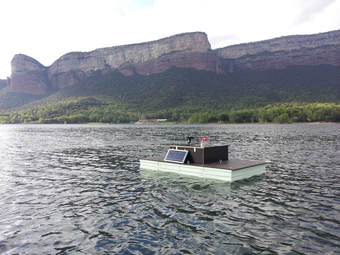
\includegraphics[width=0.49\linewidth,height=0.2\textheight]{Img/foto-sau} \includegraphics[width=0.49\linewidth,height=0.2\textheight]{Img/BoyaGergal} 

}

\caption{**Sistemas de monitoreo de alta frecuencia.** *Izquierda:* boya flotante que realiza medidas cada 10 minutos a una profundidas de 1.5 metros en el embalse de Sau (Barcelona). *Derecha:* boya flotante que realiza perfiles verticales desde la superficie hasta el fondo con un resolución espacial de 1 metro y una resolución temporal de 2 horas en el embalse de El Gergal (Sevilla).}\label{fig:unnamed-chunk-1}
\end{figure}

Los monitoreos de alta frecuencia (HFM) tienen muchas aplicaciones dentro de la ecología acuática, tanto en el ámbito de la gestión como de la investigación. Por ejemplo, pueden ser usados para controlar la calidad del agua en un embalse que suministra agua potable a una ciudad, control de vertidos de una industria, estudiar el efecto de eutrofización en un lago de alta montaña o detectar cambios en las corrientes marinas.

Sin embargo, no todo es de color de rosas. Imaginaos que, después de dos años, vamos a recoger la información que ha almacenado nuestro sensor de temperatura y oxígeno disuelto que dejamos colocado en el centro de un lago de los pirineos. Al descargar la información, nos encontramos que tenemos 1.036.800 registros (porque claro está, queríamos registrar los datos cada segundo)\ldots{} Echamos manos mano de nuestro amado Excel (Calc para los radicales del software libre) e intentamos calcular la temperatura media de esos dos años entre las 00:00 a las 08:00. A mí me ha entrado un sudor frío. Y es que, esta vasta y valiosa información tiene un inconveniente\ldots{} tenemos que trabajar con miles o millones de datos. Por suerte, se disponen de muchas herramientas para trabajar con los datos.

En esta práctica de Ecología de Sistemas Acuáticos, en la que vamos a trabajar con datos de HFM para estudiar la estructura térmica de un lago, me gustaría presentaros una herramienta, que a mi parecer, es fundamental para cualquier biólog@ y que os permitirá realizar todo el trabajo (desde organización de la información hasta su visualización, pasando por el análisis estadístico) con un solo software libre, de código abierto y gratuito. Estamos hablando de \href{https://www.r-project.org/}{R}. Para \href{mailto:l@s}{\nolinkurl{l@s}} que no lo conozcáis, Si buscáis R en google os aparecerá en las primera 4-5 entradas. Esto nos puede dar una idea de su relevancia a nivel mundial.

A partir de aquí, no os voy a engañar, R no es, por lo general, muy agradable y no suele despertar simpatías. ¡Echad un vistazo a la figura de abajo!

\begin{figure}

{\centering 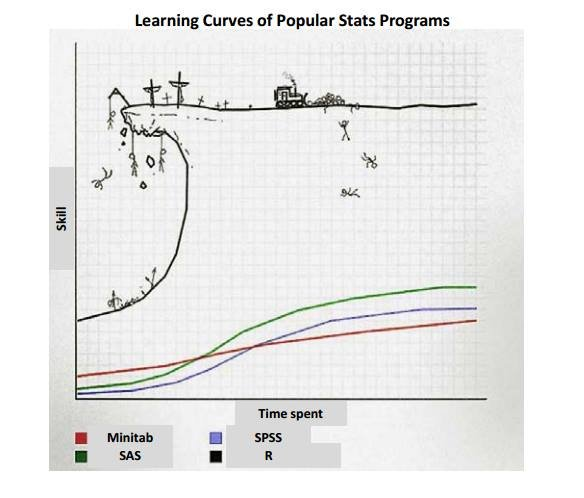
\includegraphics[width=1\linewidth]{Img/Learn_R} 

}

\caption{Comparación de la curva de aprendizaje de distintos software estadísticos. Fuente: https://twitter.com/rogierK/status/730863729420701697}\label{fig:unnamed-chunk-2}
\end{figure}

Sin embargo, cuando esos momentos de flaqueza acontezcan imaginad si sería posible hacerlo con otra herramienta y el tiempo que os llevaría. Además, cada vez que tengáis que hacer un estudio o evaluación necesitaréis usar Excel para ordenar los datos, SPSS (u otro programa de estadística) para el análisis y sigma plot (o similar) para hacer gráficas decentes. Mejor no hablamos de software específicos para cada campo: VENSIM, PRIME, Ocean Data View, SURFER, etc. A la larga el tiempo invertido habrá merecido la pena.

\hypertarget{estructura-de-la-pruxe1ctica}{%
\chapter{Estructura de la práctica}\label{estructura-de-la-pruxe1ctica}}

\begin{enumerate}
\def\labelenumi{\arabic{enumi}.}
\tightlist
\item
  \protect\hyperlink{Descarga}{Obtener los datos con los que vamos a trabajar.} Usaremos la red \href{https://gleon.org/}{The Global Lake Ecological Observatory Network (GLEON)}. Esta red pone a nuestra disposición una amplia cantidad de datos de monitoreo de alta frecuencia (HFM) de distintos lugares del mundo.
\item
  \protect\hyperlink{PrimerosPasos}{Primeros pasos en R.}
\item
  \href{@Tidyverse}{Familiarizarnos con los paquetes y funciones básicos de R que nos permiten explorar y trabajar con grandes tablas de datos.}
\item
  \href{@Termoclina}{Calcular profundidad de la termoclina y la estabilidad de la columna de agua (número de Smidch)} usando el paquete de R \href{https://cran.r-project.org/web/packages/rLakeAnalyzer/rLakeAnalyzer.pdf}{rLakeAnalyzer}.
\item
  \protect\hyperlink{Contour}{Gráficas de contorno}.
\end{enumerate}

\hypertarget{Descarga}{%
\chapter{Descargar los datos de la red GLEON}\label{Descarga}}

Para ello, visitamos la página de la red \href{https://gleon.org/}{GLEON} y nos vamos al apartado de \href{https://gleon.org/data}{datos}. En esta sección podemos encontrar la \href{https://gleon.org/sites/default/files/pdf/data/2009_October_15_GLEON_data_access_policy.pdf}{política de datos de GLEON}, básicamente se apuesta por una ciencia colaborativa en la que los datos quedan a disposición de la comunidad para cualquier fin de investigación, académico, educativo o cualquier otro, siempre que no haya un interés lucrativo detrás y respetando algunos principios de comunicación con los responsables de los datos. Como se muestra en esta sección, a los datos de GLEON se puede acceder a través de tres buscadores \href{https://portal.edirepository.org/nis/home.jsp}{EDI}, \href{https://search.dataone.org/data}{DataONE} o \href{https://datasetsearch.research.google.com/}{Google data set}.

Pues bien, para este práctica vamos a trabajar, en concreto, con datos del \href{https://lter.limnology.wisc.edu/researchsite/crystal-lake}{lago Crystal}.
Así que utilizando el buscador que más sea de vuestro agrado lanzamos la siguiente búsqueda: \emph{crystal lake}.
Entre los resultados obtenidos (hay bastante información como podéis observar), vamos a seleccionar los datos derivados del proyecto \href{https://lter.limnology.wisc.edu/index.php/}{North Temperate Lakes Long Term Ecologycal Research (NTL-LTER)} que nos ofrecen datos de temperatura, oxígeno disuelto, clorofila \emph{a} y pH desde 2011 hasta 2014. Si no pudierais encontrarlos, podéis pinchar \href{https://portal.edirepository.org/nis/mapbrowse?packageid=knb-lter-ntl.303.20}{aquí: North Temperate Lakes LTER High Frequency Water Temperature Data, Dissolved Oxygen, Chlorophyll, pH - Crystal Lake 2011 - 2014}.

En esa página que acabáis de abrir tenéis un sumario con toda la información necesario sobre el paquete de datos (\emph{Title, Creators, Publication Date, Citation, Abstract, Spatial Coverage, Package ID, Resources, Intellectual Rights, Digital Object Identifier, PASTA Identifier, Code Generation, Provenance, Journal Citations}). Las que más nos van a interesar por el momento son \emph{Abstract, Resources y Code Generation}. La primera de ellas es un resumen que nos explica como han sido recogido los datos y algunas particularidades que debemos saber, en la segunda tenemos directamente los archivos con los datos para descargarlos en formato *.csv y una opción muy interesante, \href{https://portal.edirepository.org/nis/metadataviewer?packageid=knb-lter-ntl.303.20}{\emph{View Full Metadata}}, en la que si desplegamos \emph{Data Entities} podemos ver información sobre las variables que aparecen en la tabla de datos como, por ejemplo, las unidades en las que están medidas.

En este caso, disponemos solo de un fichero. Para descargar los datos tenemos dos opciones:

\begin{enumerate}
\def\labelenumi{\arabic{enumi}.}
\tightlist
\item
  Podemos pinchar directamente en el archivo y descargarlo a través del navegador. \emph{Name:} High Resolution Water Temperature Dissolved Oxygen Chlorophyll pH - Crystal Lake \emph{File:} ntl303\_v1\_0.csv (120.5 MiB; 22 downloads). Si optamos por esta opción, posteriormente habrá que importar los datos a R.
\item
  Otra opción mucho más cómoda es la de usar un script de R que ya nos han preparado para facilitarnos la descarga e importación. Para ello, tenemos dos opciones también:
\end{enumerate}

\begin{itemize}
\tightlist
\item
  Pinchamos en el \href{https://portal.edirepository.org/nis/codeGeneration?packageId=knb-lter-ntl.117.38\&statisticalFileType=r}{icono de R} en el apartado \emph{Code Generation}.
\item
  Pinchamos en la opción \href{https://portal.edirepository.org/nis/codeGeneration?packageId=knb-lter-ntl.303.20\&statisticalFileType=tidyr}{tidyr} en el apartado \emph{Code Generation}. Os recomiendo usar esta última, es la que vemos más abajo y, además, si no lo tenemos instalado, instala automáticamente el paquete \href{https://www.tidyverse.org/}{Tidyverse}. \passthrough{\lstinline!Tidyverse!} es en realidad un conjunto de paquetes de R especialmente diseñado para la ciencia de datos que nos vendrá de maravilla para esta práctica.
\end{itemize}

Independientemente por cual os decantéis, debéis abrir el archivo pinchando en \emph{File Download: knb-lter-ntl.303.20.r} o \emph{File Download: knb-lter-ntl.303.20.tidyr} y se abrirá automáticamente con R, si no es así, lo descargáis y lo abrís posteriormente con R. Una vez abierto ya podéis ejecutar el script (\passthrough{\lstinline!Ctrl+A!} y después \passthrough{\lstinline!Crtl+Enter!}).
Como veis también hay opción para descargar y trabajar directamente los datos con otras herramientas, si a alguno le pica la curiosidad ¡adelante!. En esta práctica como hemos dicho vamos a usar R, debido a que es una herramienta gratuita, de código abierto y libre. Además es ampliamente usado en investigación debido a su naturaleza libre y colaborativa. En fin, si más dilaciones, podéis descargar el script, abrirlo con RStudio y ejecutarlo ¡A ver qué pasa!.

Esta es la pinta que tiene el script:

\begin{lstlisting}[language=R]
# Package ID: knb-lter-ntl.303.20 Cataloging System:https://pasta.edirepository.org.
# Data set title: North Temperate Lakes LTER High Frequency Water Temperature Data, Dissolved Oxygen, Chlorophyll, pH - Crystal Lake 2011 - 2014.
# Data set creator:  John Magnuson - University of Wisconsin 
# Data set creator:  Stephen Carpenter - University of Wisconsin 
# Data set creator:  Emily Stanley - University of Wisconsin 
# Data set creator:  NTL Lead PI - University of Wisconsin 
# Metadata Provider:  NTL Information Manager - University of Wisconsin 
# Contact:  NTL Information Manager -  University of Wisconsin  - ntl.infomgr@gmail.com
# Contact:  NTL Lead PI -  University of Wisconsin  - ntl.leadpi@gmail.com
# Stylesheet for metadata conversion into program: John H. Porter, Univ. Virginia, jporter@Virginia.edu 
#
#install package tidyverse if not already installed
if(!require(tidyverse)){ install.packages("tidyverse") }  
library("tidyverse") 
infile1 <- trimws("https://pasta.lternet.edu/package/data/eml/knb-lter-ntl/303/20/b9b3b932deec8f3e71fb8d70cacf6a0e") 
infile1 <-sub("^https","http",infile1)
# This creates a tibble named: dt1 
dt1 <-read_delim(infile1  
                 ,delim=","   
                 ,skip=1 
                 , col_names=c( 
                   "sampledate",   
                   "year4",   
                   "daynum",   
                   "sample_time",   
                   "depth_calculated",   
                   "wtaer_temp",   
                   "flag_water_temp",   
                   "pH",   
                   "flag_ph",   
                   "chlorophylla",   
                   "flag_chlorophylla",   
                   "opt_do2",   
                   "flag_do2",   
                   "opt_dosat_raw",   
                   "flag_opt_dosat_raw"   ), 
                 col_types=list(
                   col_character(), 
                   col_number() , 
                   col_number() , 
                   col_character(), 
                   col_number() , 
                   col_number() ,  
                   col_character(), 
                   col_number() ,  
                   col_character(), 
                   col_number() ,  
                   col_character(), 
                   col_number() ,  
                   col_character(), 
                   col_number() ,  
                   col_character()), 
                 na=c(" ",".","NA")  )


# Observed issues when reading the data. An empty list is good!
problems(dt1) 
# Here is the structure of the input data tibble: 
glimpse(dt1) 
# And some statistical summaries of the data 
summary(dt1) 
# Get more details on character variables

summary(as.factor(dt1$flag_water_temp)) 
summary(as.factor(dt1$flag_ph)) 
summary(as.factor(dt1$flag_chlorophylla)) 
summary(as.factor(dt1$flag_do2)) 
summary(as.factor(dt1$flag_opt_dosat_raw))
\end{lstlisting}

Esta primera parte del script es para descargar los datos (igual que arriba, salvo que me he tomado el tiempo de comentar algunas líneas):

\begin{lstlisting}[language=R]
# Package ID: knb-lter-ntl.303.20 Cataloging System:https://pasta.edirepository.org.
# Data set title: North Temperate Lakes LTER High Frequency Water Temperature Data, Dissolved Oxygen, Chlorophyll, pH - Crystal Lake 2011 - 2014.
# Data set creator:  John Magnuson - University of Wisconsin 
# Data set creator:  Stephen Carpenter - University of Wisconsin 
# Data set creator:  Emily Stanley - University of Wisconsin 
# Data set creator:  NTL Lead PI - University of Wisconsin 
# Metadata Provider:  NTL Information Manager - University of Wisconsin 
# Contact:  NTL Information Manager -  University of Wisconsin  - ntl.infomgr@gmail.com
# Contact:  NTL Lead PI -  University of Wisconsin  - ntl.leadpi@gmail.com
# Stylesheet for metadata conversion into program: John H. Porter, Univ. Virginia, jporter@Virginia.edu 
#
#install package tidyverse if not already installed. Aquí cargamos el conjunto de paquetes que están dentro de "tidyverse" y si no lo tuvieramos instaldo, han pensado en nosotros y, se instala solo.
if(!require(tidyverse)){ install.packages("tidyverse") }  
library("tidyverse") 
infile1 <- trimws("https://pasta.lternet.edu/package/data/eml/knb-lter-ntl/303/20/b9b3b932deec8f3e71fb8d70cacf6a0e") 
#Esta, de arriba, es la dirección de donde descarga los datos
infile1 <-sub("^https","http",infile1)
# This creates a tibble named: dt1 
dt1 <-read_delim(infile1  #Crea un objeto donde descarga los datos de la dirección que le damos, guardada en el objeto con nombre "infile1"
                 ,delim=","   
                 ,skip=1 
                 , col_names=c(        #Asigna nombre a las columnas
                   "sampledate",   
                   "year4",   
                   "daynum",   
                   "sample_time",   
                   "depth_calculated",   
                   "wtaer_temp",   
                   "flag_water_temp",   
                   "pH",   
                   "flag_ph",   
                   "chlorophylla",   
                   "flag_chlorophylla",   
                   "opt_do2",   
                   "flag_do2",   
                   "opt_dosat_raw",   
                   "flag_opt_dosat_raw"   ), 
                 col_types=list(
                   col_character(), 
                   col_number() , 
                   col_number() , 
                   col_character(), 
                   col_number() , 
                   col_number() ,  
                   col_character(), 
                   col_number() ,  
                   col_character(), 
                   col_number() ,  
                   col_character(), 
                   col_number() ,  
                   col_character(), 
                   col_number() ,  
                   col_character()), 
                 na=c(" ",".","NA")  )
\end{lstlisting}

Este trocito de código que sigue es para corregir algún problema de formato que se haya podido introducir debido a algún error en la base de datos.

\begin{lstlisting}[language=R]
# Observed issues when reading the data. An empty list is good!
problems(dt1) 
\end{lstlisting}

Este último trozo es simplemente para ver la estructura de los datos y un resumen de cada una de la variables. Este trozo no es necesario que lo ejecutéis.

\begin{lstlisting}[language=R]
# Here is the structure of the input data tibble: 
glimpse(dt1) 
# And some statistical summaries of the data 
summary(dt1) 
# Get more details on character variables

summary(as.factor(dt1$flag_water_temp)) 
summary(as.factor(dt1$flag_ph)) 
summary(as.factor(dt1$flag_chlorophylla)) 
summary(as.factor(dt1$flag_do2)) 
summary(as.factor(dt1$flag_opt_dosat_raw))
\end{lstlisting}

Bien, una vez ejecutado el script, ya debemos tener los datos en nuestro entorno de RStudio en un tipo de objeto denominado data.frame (básicamente una tabla de datos). Vamos a ver que pinta tienen:

\begin{lstlisting}[language=R]
head(dt1)
\end{lstlisting}

Por último, los vamos a guardar en la carpeta ``Datos'' que hemos creado.

\begin{lstlisting}[language=R]
write.csv(dt1, "./Datos/Datos_Crystal.csv", row.names = FALSE)
\end{lstlisting}

\hypertarget{PrimerosPasos}{%
\chapter{Primero pasos}\label{PrimerosPasos}}

A estas alturas es posible que ya se haya generado una histeria colectiva. A la mayoría de vosotr@s ya os habrá dado algún error y, a l@s que no, esa cantidad de código ininteligible os habrá quitado las ganas de vivir. ¡Que no cunda el pánico!

Vamos a ver alguna nociones básicas sobre R. Si os preguntáis porqué ahora y no antes: porque hasta que no surgen las dudas, no tiene sentido dar las respuestas.

\begin{figure}

{\centering 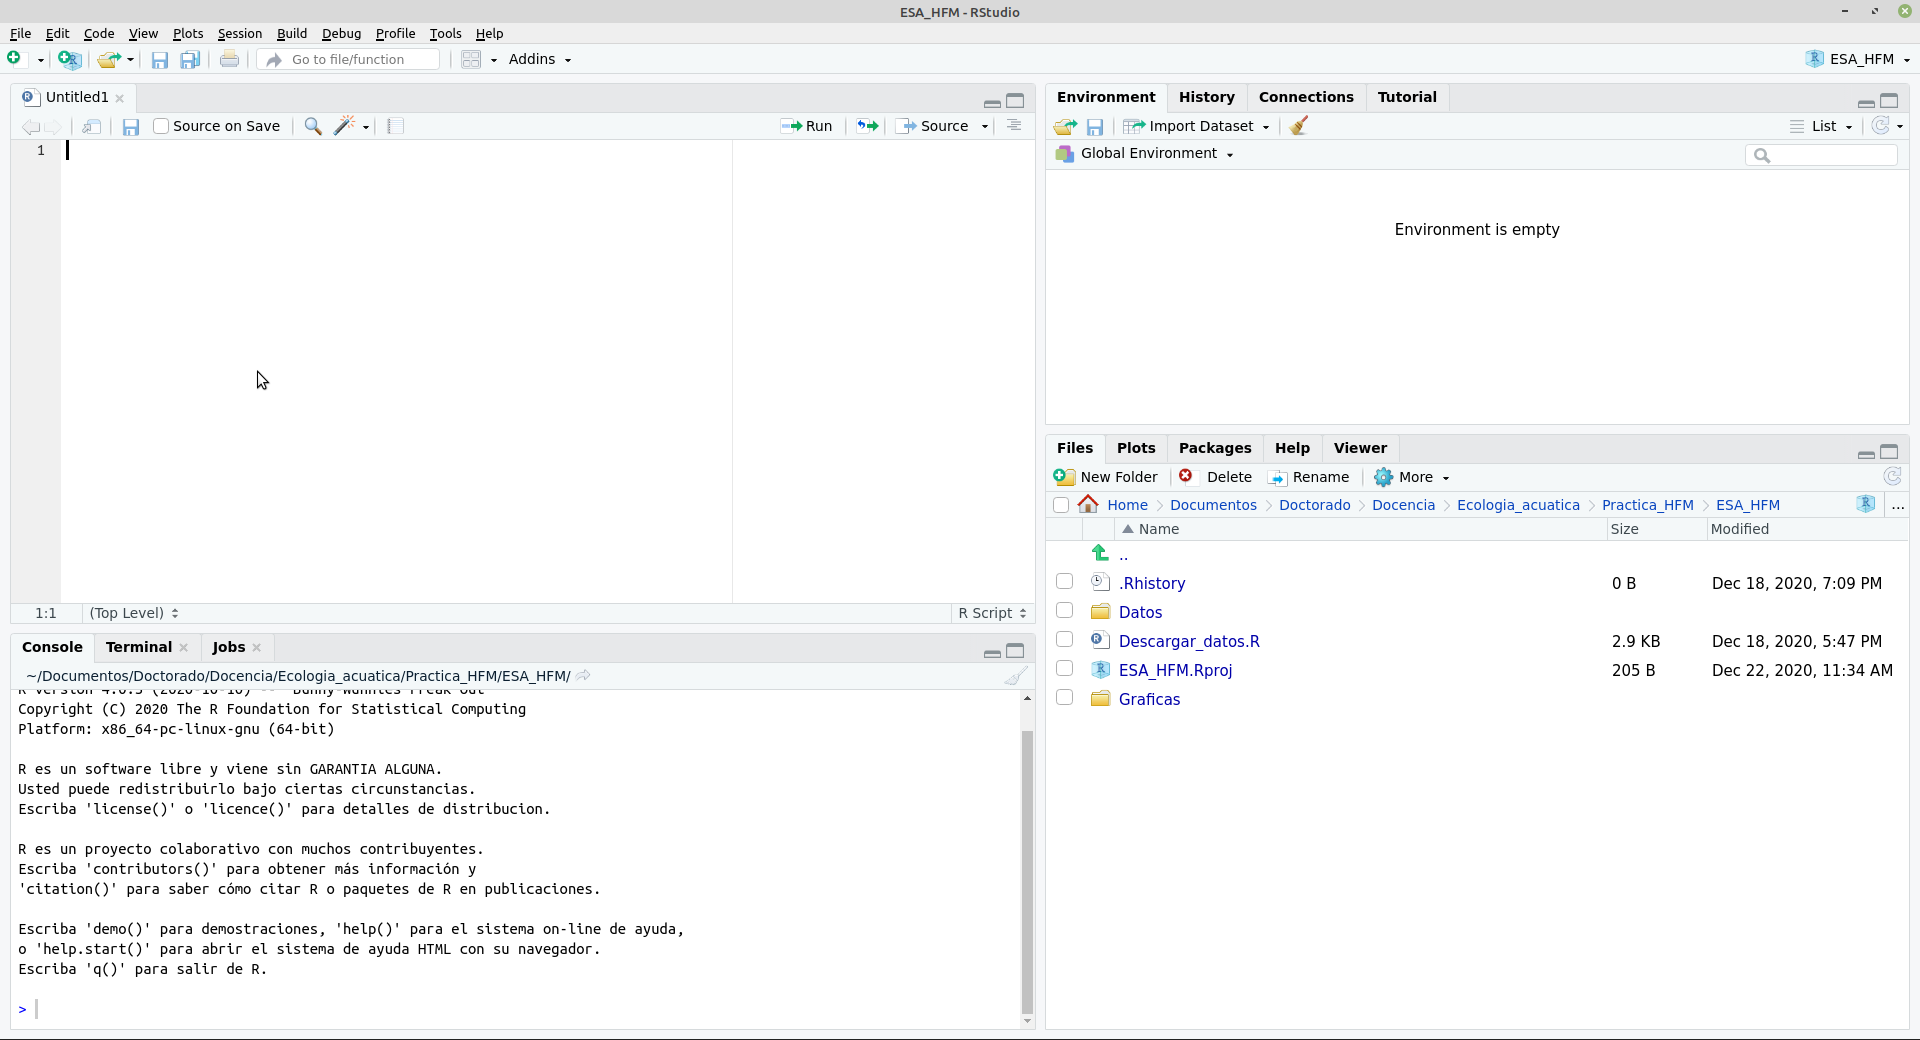
\includegraphics[width=1\linewidth]{Img/RStudio_interfaz} 

}

\caption{Interfaz de R.}\label{fig:unnamed-chunk-9}
\end{figure}

RStudio es una IDE (entorno de desarrollo integrado) para R. En román paladino, RStudio nos permite usar R de una manera más intuitiva y con muchas herramientas que nos facilitan la vida. Como vamos usar RStudio para comunicarnos con R, cada vez que hablemos de R vamos a referirnos indistintamente a R y a RStudio. Bien, pues en la imagen de arriba vemos 4 subventanas. Veamos una a una:

\begin{figure}

{\centering 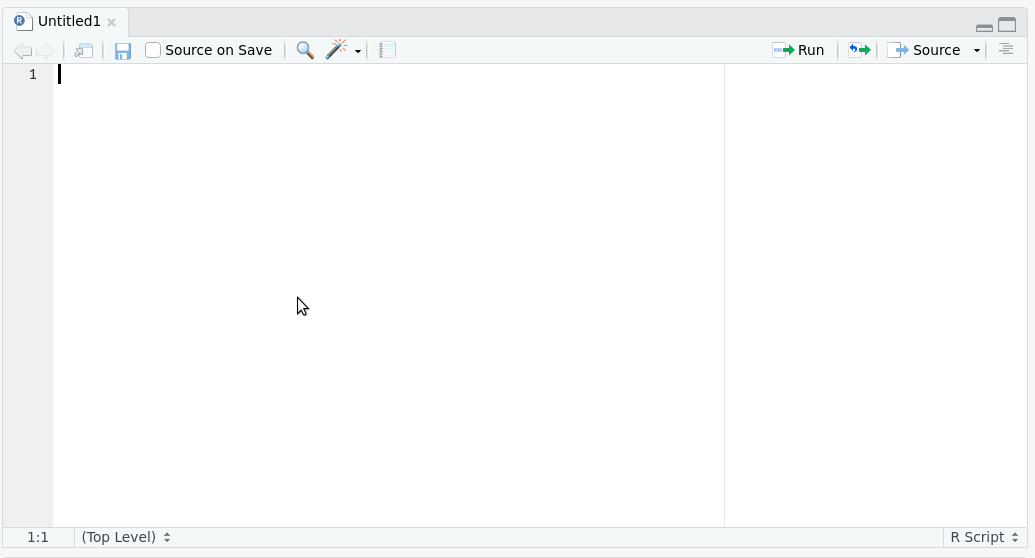
\includegraphics[width=1\linewidth]{Img/Script} 

}

\caption{Scripts en R.}\label{fig:unnamed-chunk-10}
\end{figure}

En esta ventana se muestra el script. El script no es, ni más ni menos, que una hoja donde vamos escribiendo todas las ordenes que le queremos dar a R. Nos permite ir guardando todo lo que hacemos, modificar sobre lo que ya hemos hecho, ejecutar sólo la parte que nos interesa y organizar la información. Vamos a escribir nuestra primera línea en R, usándolo como una simple calculadora (pincha sobre el recuadro \passthrough{\lstinline!code!} para ver el código):

\begin{lstlisting}[language=R]
2+2
\end{lstlisting}

\begin{lstlisting}
## [1] 4
\end{lstlisting}

Si escribís 2+2 y pulsáis \passthrough{\lstinline!Ctrl+Enter!} se ejecuta solo la línea en la que estamos. Veréis que el resultado (4) os aparece en la ventana consola:

\begin{figure}

{\centering 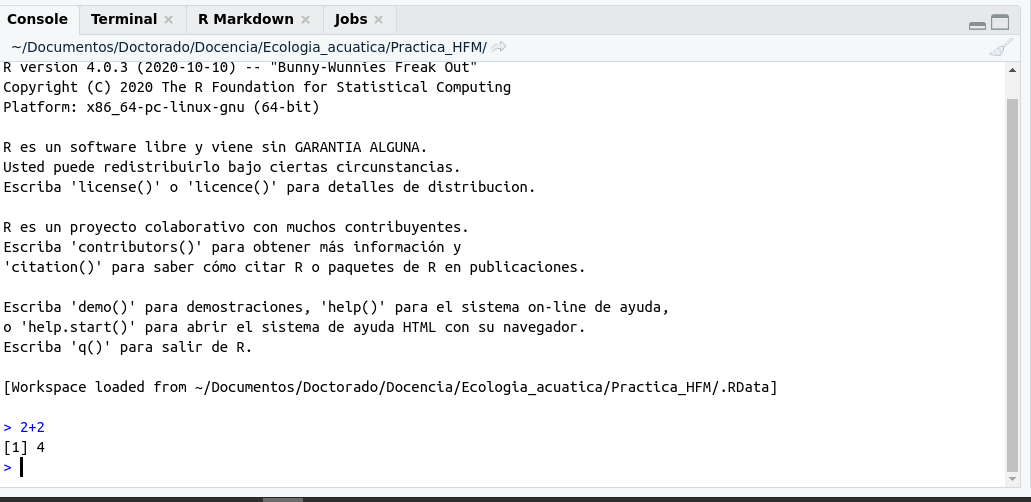
\includegraphics[width=1\linewidth]{Img/Console_R_2} 

}

\caption{Consola R.}\label{fig:unnamed-chunk-12}
\end{figure}

Como podéis intuir la consola es donde tiene lugar la parte importante. En ella se ejecutan las ordenes, nos informa de los errores y nos devuelve la información que le pedimos.

Volvamos al script. R es una lenguaje orientado a objetos, esto se traduce en que vamos a ir guardando la información en ``objetos'' virtuales y vamos a trabajar con estos objetos. Siguiente el ejemplo anterior, vamos a crear nuestros primeros objetos:

\begin{lstlisting}[language=R]
x <- 2
y <- 2
\end{lstlisting}

Hemos creado dos objetos, una llamado \passthrough{\lstinline!x!} y otro llamado \passthrough{\lstinline!y!}. Ambos guardan la información del valor 2. Además, si os habéis fijado, en la ventana superior derecha os han aparecido esos dos objetos:

\begin{figure}

{\centering 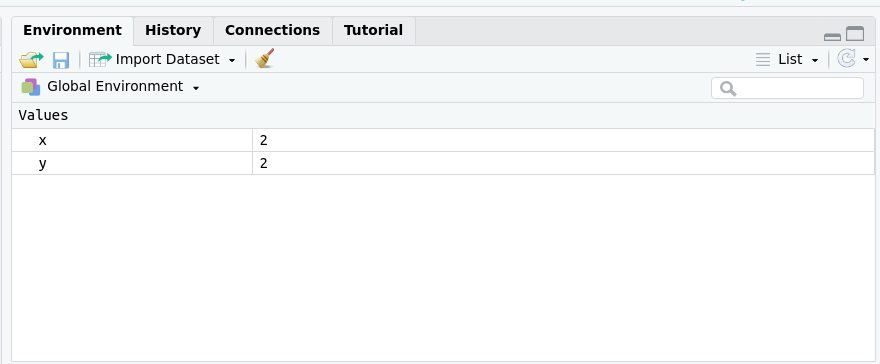
\includegraphics[width=1\linewidth]{Img/Environment_R_2} 

}

\caption{Ventana Environment.}\label{fig:unnamed-chunk-14}
\end{figure}

En esta ventana aparecerán todos los objetos que hemos creado durante nuestra sesión de trabajo.

Ahora vamos a sumar estos dos objetos:

\begin{lstlisting}[language=R]
x+y
\end{lstlisting}

\begin{lstlisting}
## [1] 4
\end{lstlisting}

¡Enhorabuena! ya habéis creado vuestros primeros objetos en R y habéis trabajado con ellos. Ahora vamos a sacarle más partido a esto. Como imaginaréis, en un objeto de R se puede almacenar muchas más información que un sólo número. Vamos a imaginar que tenemos información sobre la temperatura del agua medida en distintos sistemas epicontinentales y queremos guardar esa información en un objeto llamado \passthrough{\lstinline!Temperatura!}:

\begin{lstlisting}[language=R]
Temperatura <- c(23, 23.5, 20, 25)
\end{lstlisting}

Ahora vamos a calcular la temperatura media y su desviación:

\begin{lstlisting}[language=R]
mean(Temperatura)
\end{lstlisting}

\begin{lstlisting}
## [1] 22.875
\end{lstlisting}

\begin{lstlisting}[language=R]
sd(Temperatura)
\end{lstlisting}

\begin{lstlisting}
## [1] 2.096624
\end{lstlisting}

¡Ojo! R es muy quisquilloso y si no le dais el nombre exacto de \passthrough{\lstinline!Temperatura!} (incluyendo mayúsculas y minúsculas) no os entenderá y os devolverá un error. Por lo tanto, sed muy cuidadosos con la sintaxis y revisad que todo está escrito correctamente (que no falte ningún paréntesis o corchete).

En estas últimas líneas han sucedido un par de cosas: hemos creado un objeto nuevo, un vector, y hemos usado dos funciones \passthrough{\lstinline!mean()!} y \passthrough{\lstinline!sd()!} que calculan la media y desviación estándar.

Un vector almacena información de un mismo tipo, en este caso numérico. Existen distintos tipos de vector en función de la información que almacén:

\begin{enumerate}
\def\labelenumi{\arabic{enumi}.}
\tightlist
\item
  Numérico: almacenan números.
\item
  Carácter: almacenan texto.
\item
  Factores: almacenan factores, generalmente texto pero que usaremos como un tratamiento en el análisis.
\item
  Fechas: almacenan fechas en distintos formatos.
\end{enumerate}

En cuanto a las funciones, existen infinidad de ellas. R trae muchas funciones básicas pero si queremos aplicar funciones más especificas necesitaremos instalar paquetes que han sido creados específicamente para ello.

La estructura genérica de una función sería.

\begin{lstlisting}[language=R]
nombre_funcion(x = objeto_donde_aplicarla, argumento1 = "valor1", argumento2 = "valor2")
\end{lstlisting}

Si queremos obtener más información sobre una función y su uso podéis usar la función \passthrough{\lstinline!help("funcion\_que\_os\_interesa")!} o más cómodo \passthrough{\lstinline!?funcion\_que\_os\_interesa!}:

\begin{lstlisting}[language=R]
?mean
\end{lstlisting}

Veréis que se os abrirá la última ventana que nos quedaba por ver:

\begin{figure}

{\centering 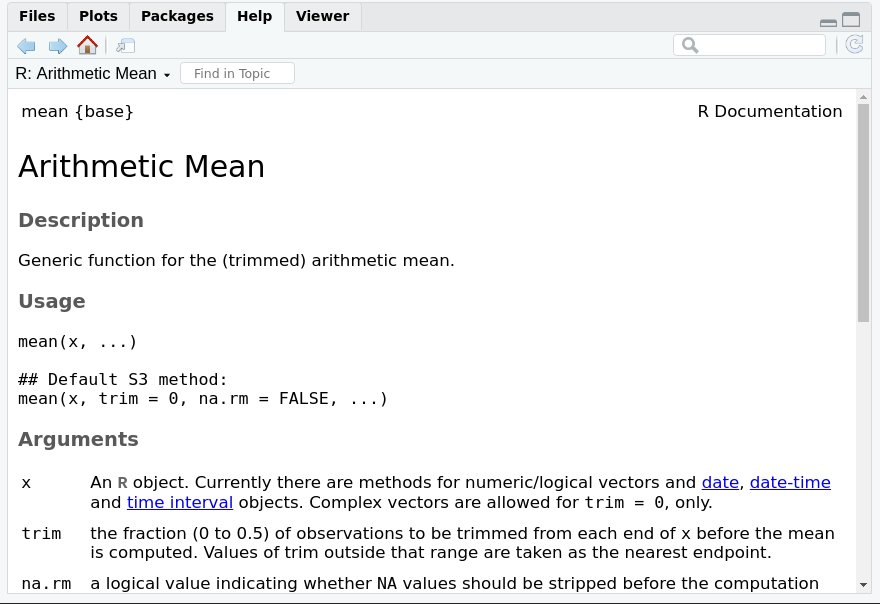
\includegraphics[width=1\linewidth]{Img/Help_R_2} 

}

\caption{Ayuda en RStudio}\label{fig:unnamed-chunk-20}
\end{figure}

Aquí encontréis la información necesaria para usar la función así como algunos ejemplos.

Por último, vamos a ver otro objeto muy útil: \passthrough{\lstinline!data.frame!}. Un data.frame no es más que una tabla de datos, como la que acostumbráis a hacer en Excel. Veamos un ejemplo:

Ya tenemos la temperatura del agua que se ha registrado en distintos sistemas epicontinentales (\passthrough{\lstinline!Temperatura!}). Ahora nos dan la información del tipo de sistema y queremos crear un tabla que recoja toda la información:

\begin{lstlisting}[language=R]
Temperatura <- c(23, 23.5, 20, 25)
Sistemas <- c("Lago", "Lago", "Rio", "Rio") #Creamos un vector esta vez de tipo caracter (el texto va entre comillas)

Temperatura_en_distintos_sistemas <- data.frame(Temperatura,
                                                   Sistemas)
View(Temperatura_en_distintos_sistemas) #La función View() nos muestra el objeto que deseemos.
\end{lstlisting}

Se os abrirá una ventana con la información recogida en el data.frame \passthrough{\lstinline!Temperatura\_en\_distintos\_sistemas!}. En este último trozo de código habéis visto un elemento nuevo: comentarios. Es altamente recomendado comentar el código que estamos escribiendo. De este modo, será mucho más claro y cuando vuelvas a abrir el script después de meses ``tu yo del futuro'' te lo agradecerá. Además si queréis compartir código con otr@s compañer@s es necesario añadir comentarios para que sepan que hacemos en cada sección. Para comentar, como habéis visto, sólo hay que añadir \passthrough{\lstinline!\#!} delante del texto y este no se ejecutará. Si no ponéis \passthrough{\lstinline!\#!} R lo entenderá como una orden y os dará error.

Otra cosa que habréis podido notar es que, aunque R nos ayuda autocompletando la frase, el nombre \passthrough{\lstinline!Temperatura\_en\_distintos\_sistemas!} no es muy funcional que se diga. Es más práctico usar nombres cortos, pero nos indiquen claramente de que se trata, a la hora de nombrar objetos en R.

A la hora de nombrar objetos en R hay algunas nombres que debemos respetar.

\begin{enumerate}
\def\labelenumi{\arabic{enumi}.}
\tightlist
\item
  Los nombres no pueden ser números o empezar con número. No podríamos usar \passthrough{\lstinline!1!} ó \passthrough{\lstinline!2!} ni \passthrough{\lstinline!2datos!}, pero sí podríamos usar \passthrough{\lstinline!datos2!}.
\item
  No se usar caracteres especiales: \#, !, @, etc.
\item
  Los espacios tampoco pueden ser usado dentro de los nombres. Usar en su lugar mayúsculas ó barra baja. Por ejemplo, usar \passthrough{\lstinline!DatosLagos!} o \passthrough{\lstinline!Datos\_lagos!} en lugar de \passthrough{\lstinline!Datos lagos!}.
\end{enumerate}

\begin{lstlisting}[language=R]
Temperatura <- c(23, 23.5, 20, 25)
Sistemas <- c("Lago", "Lago", "Rio", "Rio") #Creamos un vector esta vez de tipo caracter (el texto va entre comillas)

Temp_sistemas <- data.frame(Temperatura,
                                                   Sistemas)
View(Temperatura_en_distintos_sistemas) #La función View() nos muestra el objeto que deseemos.
\end{lstlisting}

¡Genial! Ya hemos visto los objetos básicos. Irán saliendo más a lo largo de la práctica, pero por ahora es suficiente.

\hypertarget{ejercicios}{%
\section{Ejercicios}\label{ejercicios}}

\begin{enumerate}
\def\labelenumi{\arabic{enumi}.}
\tightlist
\item
  \emph{¿Qué sucede si corremos \passthrough{\lstinline!Sistemas[2]!}? Prueba con distintos números.}
\item
  \emph{¿Y si corremos Temp\_sistemas{[}2{]}? Da error\ldots{} prueba Temp\_sistemas{[},2{]} ¿Y si ponemos un número delante de la \passthrough{\lstinline!,!}? ¿Que indican los números que van delante de la coma y los que van detrás?}
\item
  \emph{Además de la temperatura se midió el pH: 7.8, 7.5, 9 y 8.5. Incluye estos valores en el data.frame \passthrough{\lstinline!Temp\_sistemas!}. Hazlo con los conocimientos que tienes y luego prueba con la función \passthrough{\lstinline!cbind()!}.}
\item
  \emph{Nos dan también la concentración de clorofila a, pero en este caso falta un dato y lo rellenamos con \passthrough{\lstinline!NA!}, que significa que no está disponible. \passthrough{\lstinline!Cla <- c(15.6, NA, 3, 4)!}. Calcula la concentración de clorofila media. Recuerda, cuando tengas dudas sobre como utilizar una función: \passthrough{\lstinline!?mean!}.}
\end{enumerate}

\hypertarget{Tidyverse}{%
\chapter{Paquetes importantes y sus funciones básicas}\label{Tidyverse}}

Ya hemos dado nuestros primeros pasos en R, conocemos su entorno RStudio, hemos creado nuestros primeros objetos y aplicado un par de funciones básicas. Ahora vamos a dar un paso más allá y vamos a ver algunos de lo más paquetes que pueden ser más importantes para nosotros y sus funciones más útiles.

Para esta parte de la práctica ya debemos haber descargado los datos de la plataforma GLEON como se indicó en la \protect\hyperlink{Descarga}{sección 3}.

Lo primero que nos preguntaremos, ¿Qué es un paquete? Un paquete de R es un conjunto de funciones que han sido creadas con un objetivo común, por ejemplo hacer gráficas, y que han sido agrupadas para que puedan ser cargadas en R todas juntas.

Para instalar un paquete no tenemos mas que ejecutar:

\begin{lstlisting}[language=R]
install.packages("nombre_del_paquete")
\end{lstlisting}

\hypertarget{importar-datos}{%
\section{Importar datos}\label{importar-datos}}

La mayoría de los paquetes que vamos a ver durante la práctica han sido agrupados en una colección de paquetes que nos permite instalarlos y cargarlos todos juntos. Esta colección de paquetes se llama \href{https://www.tidyverse.org/}{\emph{tidyverse}}. El primer paquete que vamos a ver es \href{https://cran.r-project.org/web/packages/readr/readr.pdf}{\passthrough{\lstinline!readr!}}.
Si aún no hemos instalado \passthrough{\lstinline!tydiverse!}:

\begin{lstlisting}[language=R]
install.packages("tidyverse")
\end{lstlisting}

Si ya lo tenemos instalado, solo tenemos que ``llamarlo'' o cargarlo. Cada vez que abrimos una sesión de R hay que cargar los paquetes que vayamos a usar durante la sesión. No es necesario volver a instalarlos pero sí hay que cargarlos usando la función \passthrough{\lstinline!library()!}:

\begin{lstlisting}[language=R]
#Library. Al principio de nuestro scrip creamos un apartado donde iremos cargando los paquetes nos irán haciendo falta.
library(readr) #Si solo quisieramos cargar el paquete readr.
\end{lstlisting}

\begin{lstlisting}[language=R]
#Library. Al principio de nuestro scrip creamos un apartado donde iremos cargando los paquetes nos irán haciendo falta.
library(tidyverse) #De esta forma, todos los paquetes que agrupa tydiverse: ggplot2, readr, dplyr, etc. Yo usaría esta.
\end{lstlisting}

\begin{lstlisting}
## -- Attaching packages --------------------------------------- tidyverse 1.3.0 --
\end{lstlisting}

\begin{lstlisting}
## v ggplot2 3.3.2     v purrr   0.3.4
## v tibble  3.0.4     v dplyr   1.0.2
## v tidyr   1.1.2     v stringr 1.4.0
## v readr   1.4.0     v forcats 0.5.0
\end{lstlisting}

\begin{lstlisting}
## -- Conflicts ------------------------------------------ tidyverse_conflicts() --
## x dplyr::filter() masks stats::filter()
## x dplyr::lag()    masks stats::lag()
\end{lstlisting}

Vemos que al cargar \passthrough{\lstinline!tydiverse!} nos informa de qué paquetes han sido cargados y algunas funciones que tienen conflicto con otros paquetes.
Una vez cargado el paquete, la primera función que vamos a necesitar es \passthrough{\lstinline!read\_csv()!}. Esta función nos permite importar tablas que se han guardado en formato \passthrough{\lstinline!.csv!}. Al principio de la práctica, creamos un proyecto de R, descargamos los datos de la plataforma y los guardamos en la carpeta \passthrough{\lstinline!Datos!} de nuestro directorio. Si guardasteis vuestro espacio de trabajo al salir, tendréis un objeto llamado \passthrough{\lstinline!dt1!}. Pero si no guardasteis, tendremos que importar los datos de nuevo y, además, aprovechamos para ponerle un nombre que nos sea más evocador que \passthrough{\lstinline!dt1!}, usaremos, por ejemplo, \passthrough{\lstinline!Crystal!}:

\begin{lstlisting}[language=R]
Crystal <- read_csv("Datos/Datos_Crystal.csv")
\end{lstlisting}

\begin{lstlisting}
## 
## -- Column specification --------------------------------------------------------
## cols(
##   sampledate = col_datetime(format = ""),
##   year4 = col_double(),
##   daynum = col_double(),
##   sample_time = col_double(),
##   depth_calculated = col_double(),
##   wtaer_temp = col_double(),
##   flag_water_temp = col_logical(),
##   pH = col_double(),
##   flag_ph = col_logical(),
##   chlorophylla = col_double(),
##   flag_chlorophylla = col_character(),
##   opt_do2 = col_double(),
##   flag_do2 = col_logical(),
##   opt_dosat_raw = col_double(),
##   flag_opt_dosat_raw = col_logical()
## )
\end{lstlisting}

\begin{lstlisting}
## Warning: 10065 parsing failures.
##   row                col           expected actual                      file
## 41821 flag_opt_dosat_raw 1/0/T/F/TRUE/FALSE      C 'Datos/Datos_Crystal.csv'
## 41822 flag_opt_dosat_raw 1/0/T/F/TRUE/FALSE      C 'Datos/Datos_Crystal.csv'
## 41823 flag_opt_dosat_raw 1/0/T/F/TRUE/FALSE      C 'Datos/Datos_Crystal.csv'
## 41824 flag_opt_dosat_raw 1/0/T/F/TRUE/FALSE      C 'Datos/Datos_Crystal.csv'
## 41825 flag_opt_dosat_raw 1/0/T/F/TRUE/FALSE      C 'Datos/Datos_Crystal.csv'
## ..... .................. .................. ...... .........................
## See problems(...) for more details.
\end{lstlisting}

Al importar el archivo, la función reconoce automáticamente el tipo de elementos que se guarda en cada columna. Por ejemplo, la columna sampledate es de tipo fecha, mientras que year y depth\_calculated son \passthrough{\lstinline!doubles!} que vienen a ser valores numéricos no enteros (double no es más que la forma en la que ese número se expresa en forma binaria usando 64 bits).

No os preocupéis por el aviso (warnings) que nos da, nos avisa de que esperaba encontrar un tipo de valor en una columna que no se corresponde con lo que ha entrado. A nosotros no nos preocupa la información que hay en esa columna \footnote{Si no sabéis que información guarda esa columna, acordaos de que podéis mirar en los metadatos de la página donde descargasteis los datos.}.

Vamos a ver un resumen de la información que tenemos disponible en la tabla de datos.

\begin{lstlisting}[language=R]
#Vistazo general
summary(Crystal)
\end{lstlisting}

\begin{lstlisting}
##    sampledate                      year4          daynum       sample_time    
##  Min.   :2011-04-29 17:54:00   Min.   :2011   Min.   : 82.0   Min.   :   0    
##  1st Qu.:2011-10-30 02:06:45   1st Qu.:2011   1st Qu.:161.0   1st Qu.: 600    
##  Median :2012-09-26 16:19:30   Median :2012   Median :208.0   Median :1203    
##  Mean   :2013-01-11 09:27:48   Mean   :2012   Mean   :209.3   Mean   :1183    
##  3rd Qu.:2013-11-08 16:38:15   3rd Qu.:2013   3rd Qu.:257.0   3rd Qu.:1803    
##  Max.   :2014-11-04 06:42:00   Max.   :2014   Max.   :323.0   Max.   :2359    
##                                                               NA's   :758072  
##  depth_calculated   wtaer_temp    flag_water_temp       pH        
##  Min.   : 0.000   Min.   : 0.00   Mode:logical    Min.   : 0.000  
##  1st Qu.: 1.000   1st Qu.: 9.79   NA's:1049068    1st Qu.: 7.390  
##  Median : 1.000   Median :16.77                   Median : 7.930  
##  Mean   : 4.316   Mean   :15.76                   Mean   : 8.028  
##  3rd Qu.: 7.000   3rd Qu.:21.32                   3rd Qu.: 8.660  
##  Max.   :19.000   Max.   :27.41                   Max.   :12.020  
##                                                                   
##  flag_ph         chlorophylla   flag_chlorophylla     opt_do2      
##  Mode:logical   Min.   : 0.00   Length:1049068     Min.   : 0.000  
##  NA's:1049068   1st Qu.: 1.59   Class :character   1st Qu.: 8.230  
##                 Median : 2.45   Mode  :character   Median : 8.810  
##                 Mean   : 2.87                      Mean   : 8.737  
##                 3rd Qu.: 3.57                      3rd Qu.: 9.840  
##                 Max.   :10.00                      Max.   :15.690  
##                 NA's   :76577                                      
##  flag_do2       opt_dosat_raw    flag_opt_dosat_raw
##  Mode:logical   Min.   :  1.00   Mode:logical      
##  NA's:1049068   1st Qu.: 90.30   NA's:1049068      
##                 Median :100.50                     
##                 Mean   : 94.27                     
##                 3rd Qu.:104.60                     
##                 Max.   :148.50                     
##                 NA's   :10065
\end{lstlisting}

R nos muestra para cada columna los valores mínimos, máximos, la media, la mediana y los cuartiles 1 y 3. Además, también nos dice cuantos valores faltan (NA's). Recordad que podéis usar la función \passthrough{\lstinline!View()!} para ver los datos directamente, también podéis hacer doble click sobre el objeto \passthrough{\lstinline!dt1!}.

\hypertarget{organizar-tablas}{%
\section{Organizar tablas}\label{organizar-tablas}}

Una cosa está clara, tenemos mucha información y, además, el archivo es bastante pesado, casi 140 MB. Vamos a centrarnos sólo en un año, 2012 por ejemplo. Para ello vamos a tirar mano de otro paquete: \passthrough{\lstinline!dplyr!}. Este es otro de los que ya viene preparado con \passthrough{\lstinline!tidyverse!}, por lo que tendremos que cargarlo. Este paquete es muy útil para organizar, filtrar y transformar la información de las tablas, aquí os dejo un ``chuleta'' con las funciones principales: \href{https://raw.githubusercontent.com/rstudio/cheatsheets/master/data-transformation.pdf}{chuleta dplyr}. Como queremos filtrar los datos y quedarnos solo con los del año 2012, vamos a usar la función \passthrough{\lstinline!filter()!}.

\begin{lstlisting}[language=R]
#Nos quedamos sólo con los datos del 2012
Crystal_2012 <- filter(Crystal, year4 == 2012)
rm(Crystal) #Aprovechamos para eliminar el otro objeto que no nos va a servir.
\end{lstlisting}

Además, si no os fijasteis antes, el nombre de la columna que recoge la temperatura del agua está mal escrito, pone \passthrough{\lstinline!wtaer\_temp!} en lugar de \passthrough{\lstinline!water\_temp!}, como cabría esperar. Vamos a cambiárselo usando el paquete \passthrough{\lstinline!dplyr!}.

\begin{lstlisting}[language=R]
Crystal_2012 <- rename(Crystal_2012, water_temp = wtaer_temp)
\end{lstlisting}

\hypertarget{ejercicios-1}{%
\subsection{Ejercicios:}\label{ejercicios-1}}

\begin{enumerate}
\def\labelenumi{\arabic{enumi}.}
\tightlist
\item
  \emph{Filtra la tabla para quedarte con los datos del 2013.}
\item
  \emph{Filtra la tabla para quedarte solo con los datos que fueron tomados a un metro de profundidad.}
\end{enumerate}

\hypertarget{gruxe1ficas}{%
\section{Gráficas}\label{gruxe1ficas}}

¡Perfecto! Ahora vamos a hacer alguna gráfica. Para ello vamos a usar otro paquete, también incluido en tidyverse, \passthrough{\lstinline!ggplot2!}. Aquí os dejo otra chuleta para usar este paquete (\href{https://raw.githubusercontent.com/rstudio/cheatsheets/master/data-visualization-2.1.pdf}{pincha aquí}). ¿Habrá cambios en la temperatura del agua a lo largo del año? Echemos un vistazo:

\begin{lstlisting}[language=R]
ggplot(Crystal_2012, aes(x = sampledate, y= water_temp))+ #Aquí indicamos donde está la información que queremos representar (Crystal_2012) y que variables x e y
  geom_point() #Aquí indicamos el tipo de gráfico, en este caso hemos elegido puntos
\end{lstlisting}

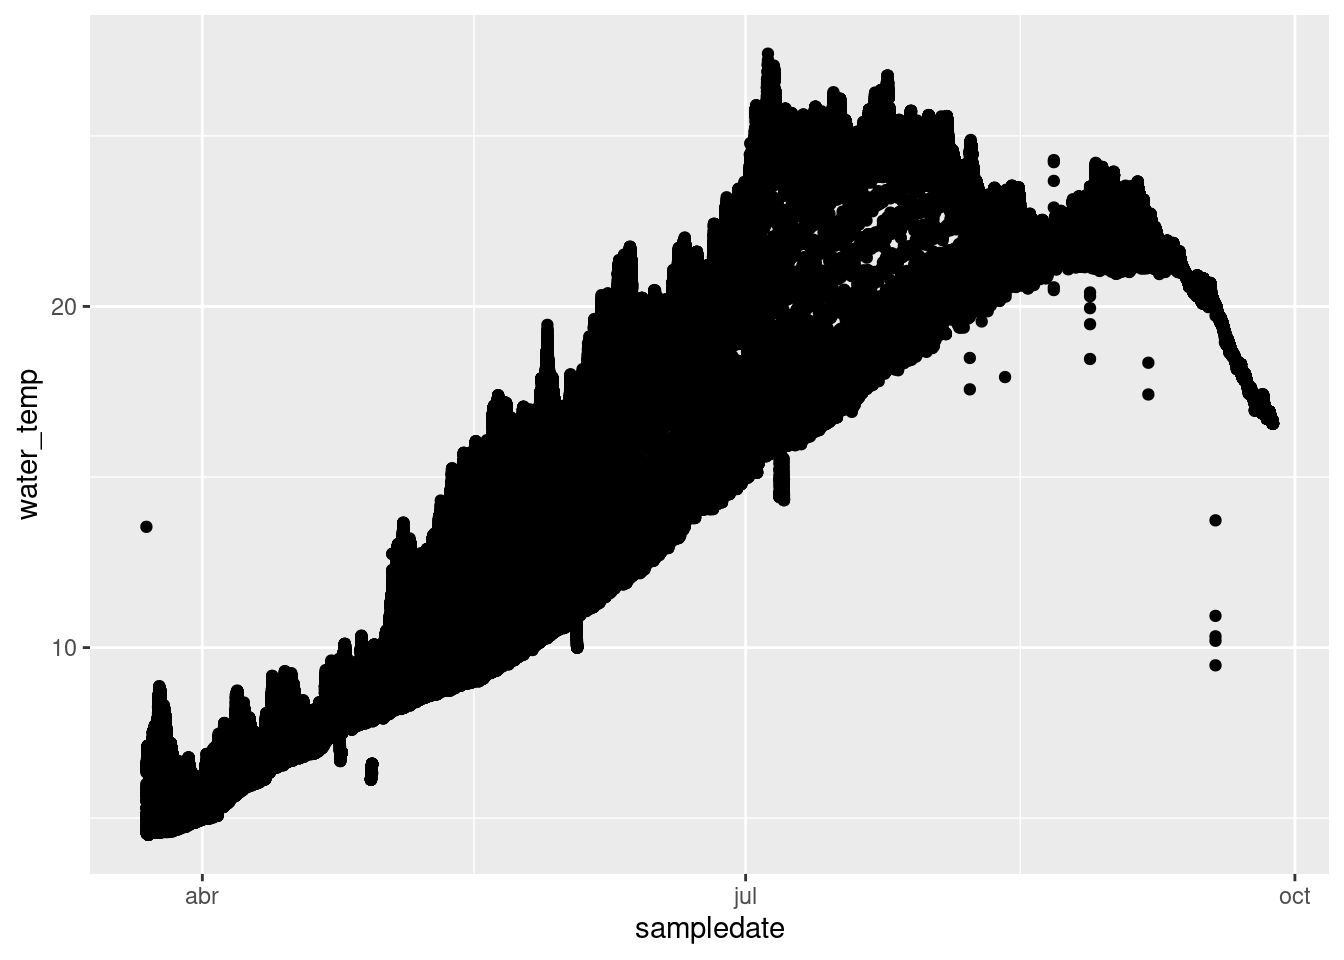
\includegraphics[width=1\linewidth]{Prácticas-Ecología-Sistemas-Acuáticos_files/figure-latex/unnamed-chunk-31-1}

Ummm\ldots{} El gráfico es un poco extraño. ¿Y si seleccionamos sólo la temperatura que tenemos a 1 metro de profundidad?

\begin{lstlisting}[language=R]
Crystal_temp_1m <- filter(Crystal_2012, depth_calculated == 1)
ggplot(Crystal_temp_1m, aes(x = sampledate, y= water_temp))+
  geom_point()
\end{lstlisting}

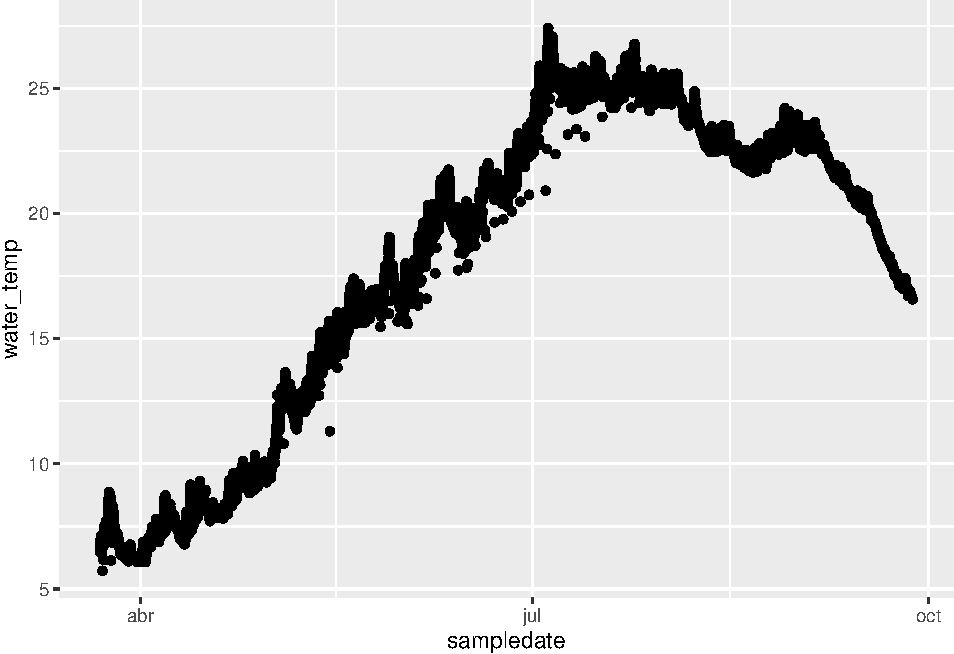
\includegraphics[width=1\linewidth]{Prácticas-Ecología-Sistemas-Acuáticos_files/figure-latex/unnamed-chunk-32-1}

Algo mejor. Vemos que la temperatura aumenta durante la primavera y que vuelve a caer cuando se entra en el otoño. Sin embargo, a parte del patrón general, se puede observar un patrón secundario. Quizás se deba a oscilaciones diarias. Para ver eso tenemos que seleccionar la temperatura a la profundidad de 1 metros y un solo día. Con la función filter podemos hacer eso.

\begin{lstlisting}[language=R]
Temp_1m_1dia <- filter(Crystal_2012, depth_calculated == 1 & daynum == 260) #Yo he elegido el día 260 (16 de septiembre)
ggplot(Temp_1m_1dia, aes(x=sampledate, y = water_temp))+
  geom_point()
\end{lstlisting}

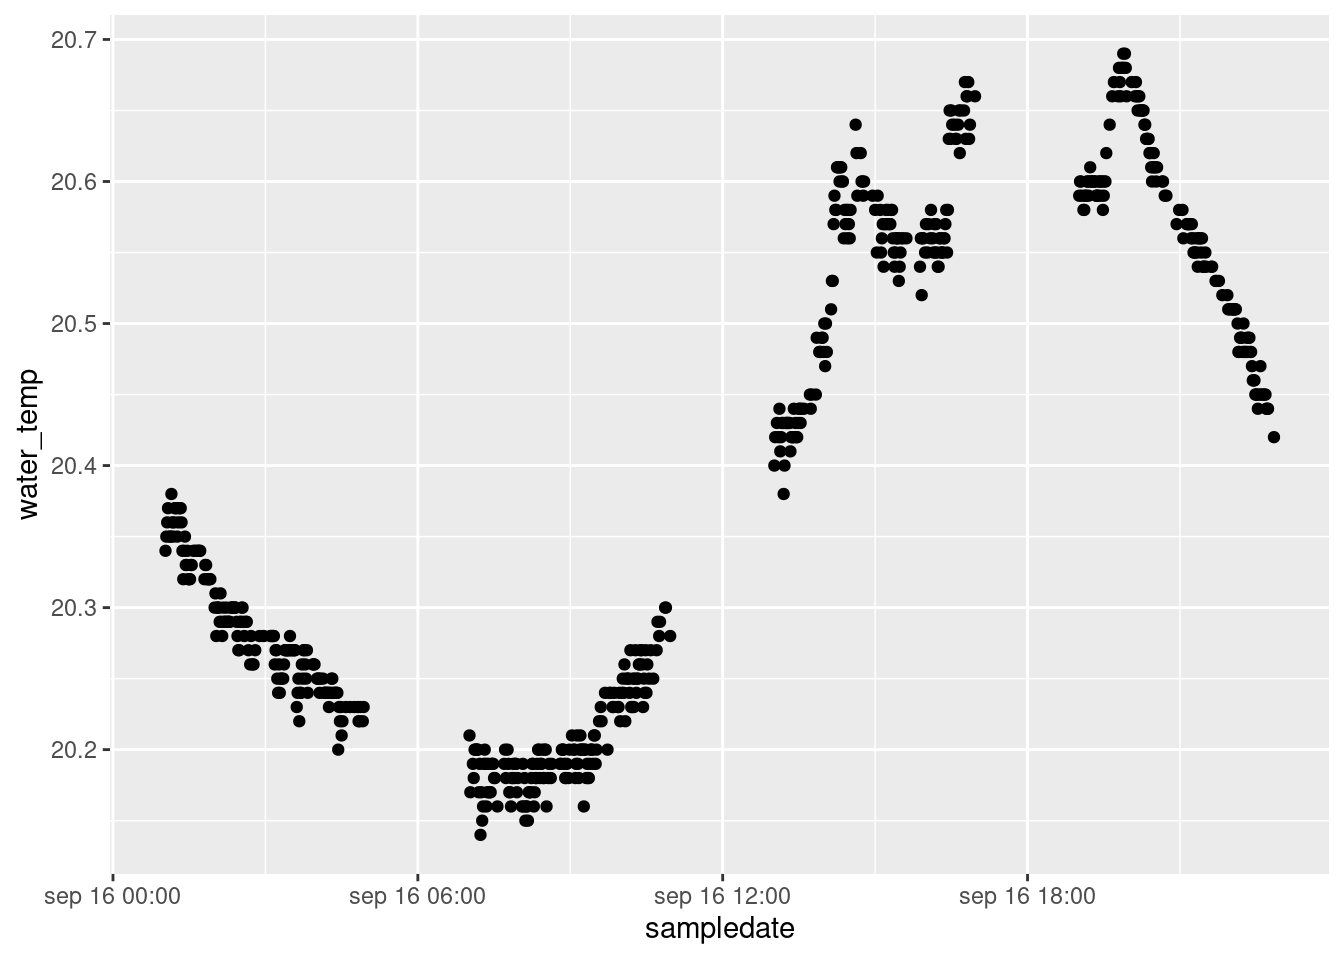
\includegraphics[width=1\linewidth]{Prácticas-Ecología-Sistemas-Acuáticos_files/figure-latex/unnamed-chunk-33-1}

Parece que sí, como cabría esperar la temperatura baja por la noche y sube por el día. Además hemos aprendido una cosa nueva en R: los operadores. Os dejo los más comunes:

\begin{longtable}[]{@{}ll@{}}
\toprule
\begin{minipage}[b]{0.14\columnwidth}\raggedright
Operador\strut
\end{minipage} & \begin{minipage}[b]{0.31\columnwidth}\raggedright
Descripción\strut
\end{minipage}\tabularnewline
\midrule
\endhead
\begin{minipage}[t]{0.14\columnwidth}\raggedright
\textgreater{}\strut
\end{minipage} & \begin{minipage}[t]{0.31\columnwidth}\raggedright
mayor que\strut
\end{minipage}\tabularnewline
\begin{minipage}[t]{0.14\columnwidth}\raggedright
\textless{}\strut
\end{minipage} & \begin{minipage}[t]{0.31\columnwidth}\raggedright
menor que\strut
\end{minipage}\tabularnewline
\begin{minipage}[t]{0.14\columnwidth}\raggedright
\textgreater=\strut
\end{minipage} & \begin{minipage}[t]{0.31\columnwidth}\raggedright
mayor o igual que\strut
\end{minipage}\tabularnewline
\begin{minipage}[t]{0.14\columnwidth}\raggedright
\textless=\strut
\end{minipage} & \begin{minipage}[t]{0.31\columnwidth}\raggedright
menor o igual que\strut
\end{minipage}\tabularnewline
\begin{minipage}[t]{0.14\columnwidth}\raggedright
==\strut
\end{minipage} & \begin{minipage}[t]{0.31\columnwidth}\raggedright
exactamente igual que\strut
\end{minipage}\tabularnewline
\begin{minipage}[t]{0.14\columnwidth}\raggedright
!=\strut
\end{minipage} & \begin{minipage}[t]{0.31\columnwidth}\raggedright
distinto a\strut
\end{minipage}\tabularnewline
\begin{minipage}[t]{0.14\columnwidth}\raggedright
x \& y\strut
\end{minipage} & \begin{minipage}[t]{0.31\columnwidth}\raggedright
x e y\strut
\end{minipage}\tabularnewline
\begin{minipage}[t]{0.14\columnwidth}\raggedright
x \textbar{} y\strut
\end{minipage} & \begin{minipage}[t]{0.31\columnwidth}\raggedright
x o y\strut
\end{minipage}\tabularnewline
\bottomrule
\end{longtable}

Ahora, vamos a hacer algunos arreglos estéticos (cambiar el nombre de los ejes, el fondo)

\begin{lstlisting}[language=R]
ggplot(Temp_1m_1dia, aes(x = sampledate, y= water_temp))+ #Aquí indicamos donde está la información que queremos representar (Crystal_2012) y qué variables x e y
  geom_point()+ #Aquí indicamos el tipo de gráfico, en este caso hemos elegido puntos
  labs(x = "Fecha", y = "Temperatura", title = "Temperatura a 1 m de profundidad")+ #Aquí  podemos modificar las etiquetas del gráfico.
  theme_classic() #Esta función usa un "tema" predefinido para la gráfica
\end{lstlisting}

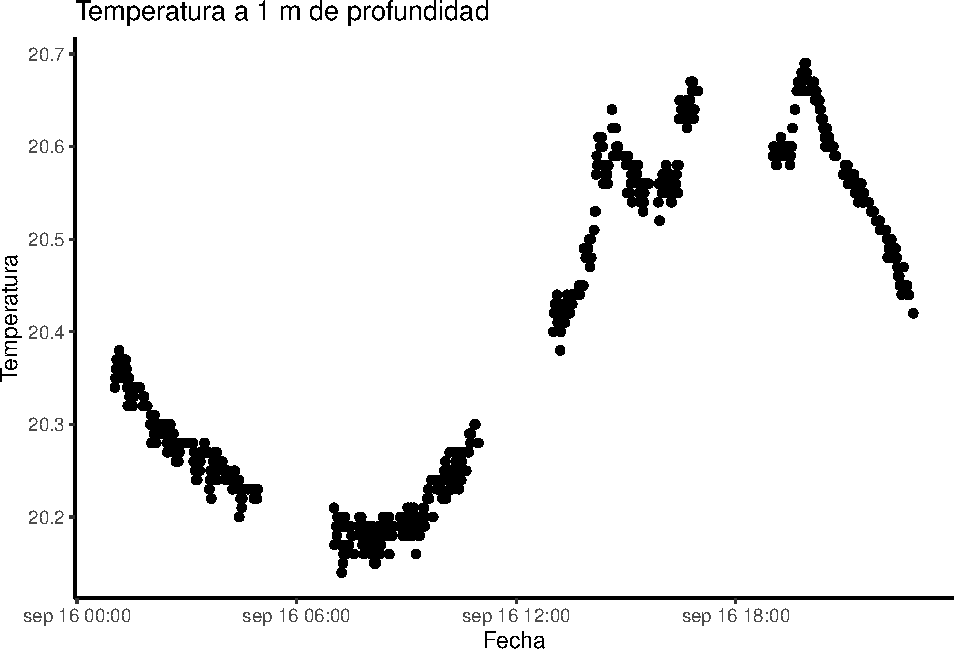
\includegraphics[width=1\linewidth]{Prácticas-Ecología-Sistemas-Acuáticos_files/figure-latex/unnamed-chunk-34-1}

Ya tiene mejor pinta. Vamos a ver si se comporta igual a distinta profundidad. Para ello, solo tenemos que decirle a ggplot que nos haga una gráfica por cada profundidad usando \passthrough{\lstinline!facet\_wrap()!}.

\begin{lstlisting}[language=R]
Crystal_temp_dia260 <- filter(Crystal_2012, daynum == 260)
ggplot(Crystal_temp_dia260, aes(x = sampledate, y= water_temp))+ #Aquí indicamos donde está la información que queremos representar (Crystal_2012) y que variables x e y
  geom_point()+ #Aquí indicamos el tipo de gráfico, en este caso hemos elegido puntos
  labs(x = "Fecha", y = "Temperatura", title = "Temperatura a 1 m de profundidad")+ #Aquí  podemos modificar las etiquetas del gráfico.
  facet_wrap(~depth_calculated)+ #En esta línea le indicamos que haga una gráfica por cada profundidad.
  scale_x_datetime(date_labels = "%R")+ #He añadido esta línea para que el formato de la fecha ponga solo la hora.
  theme_classic() #Esta función usa un "tema" predefinido para la gráfica
\end{lstlisting}

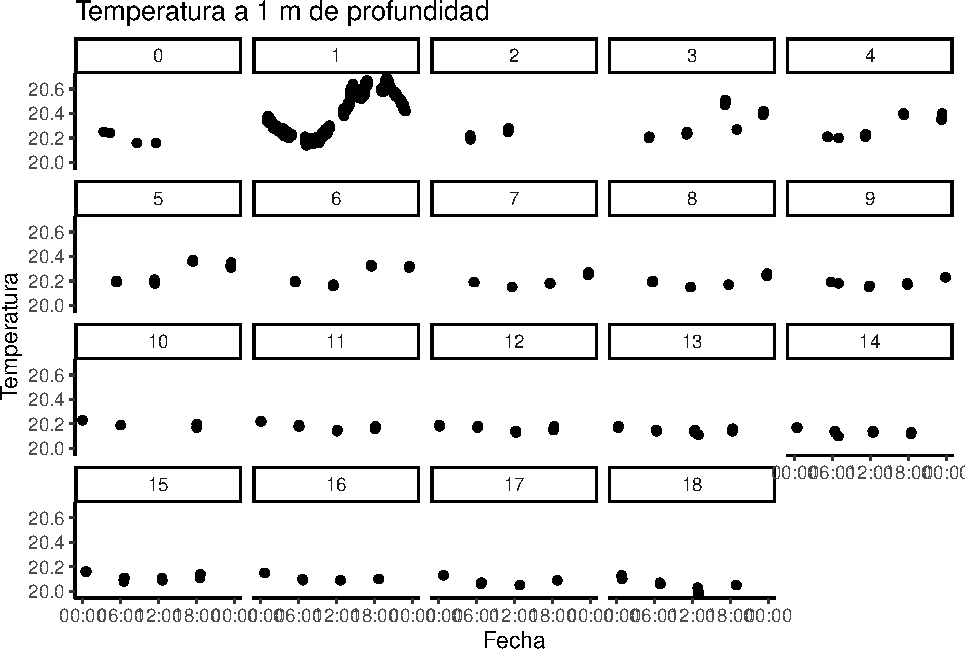
\includegraphics[width=1\linewidth]{Prácticas-Ecología-Sistemas-Acuáticos_files/figure-latex/unnamed-chunk-35-1}

Aquí podemos ver varias cosas interesantes. Por un lado, la temperatura parece oscilar a lo largo del día (día-noche) sólo en las capas más superficiales pero en las capas profundas la variación es mínima ¿alguna idea? ¿Podría estar la masa de agua estratificada? Lo veremos más adelante\ldots{} Por otro lado, vemos que la cantidad de información (puntos) no es la misma en cada profundidad, a 1 metros tenemos muchos más registros de temperatura que a 10 o 12 metros. Vamos a comprobar si es algo general para todos los días:

\begin{lstlisting}[language=R]
#Contamos el número de filas que hay para cada profundidad y día
Test_profundidades <- Crystal_2012 %>% group_by(daynum, depth_calculated) %>% summarise(n_filas = n())
\end{lstlisting}

\begin{lstlisting}
## `summarise()` regrouping output by 'daynum' (override with `.groups` argument)
\end{lstlisting}

\begin{lstlisting}[language=R]
#Lo representamos en una gráfica
ggplot(Test_profundidades, aes(x = depth_calculated, y = n_filas))+
  geom_point()+
  labs(x = "Profundidad", y = "Número de filas")+
  theme_classic()
\end{lstlisting}

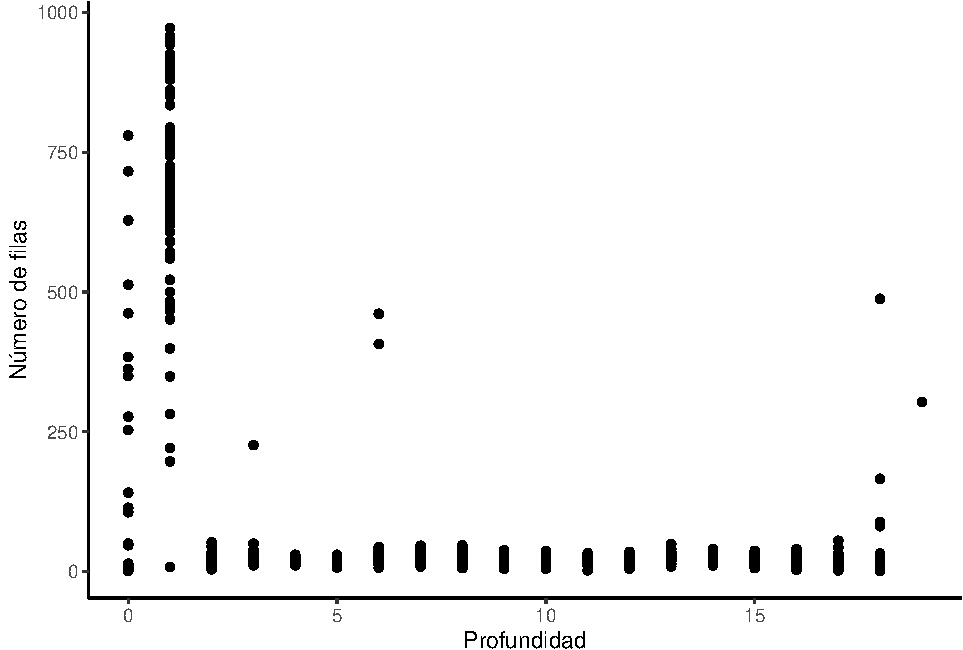
\includegraphics[width=1\linewidth]{Prácticas-Ecología-Sistemas-Acuáticos_files/figure-latex/unnamed-chunk-36-1}

Vemos que en las profundidades de 0 metros y 1 metro hay muchos más registros que en el resto. Por lo tanto, la variabilidad diaria puede no estar igual de bien recogida para todas las profundidades. En la siguiente sección vamos a seleccionar una franja horaria y a obtener un valor medio por profundidad.

En el código que acabamos de ejecutar habréis encontrado algunos elementos nuevos. Tres funciones nuevas, \passthrough{\lstinline!group\_by()!}, \passthrough{\lstinline!summarise()!} y \passthrough{\lstinline!n()!}, que nos permiten agrupar en función de las variables que queramos, resumir la información de la tabla y contar el número de elementos que hay en un grupo, respectivamente. Y un nuevo operador denominado ``pipe'', \passthrough{\lstinline!\%>\%!}. El operador \passthrough{\lstinline!\%>\%!} nos permite concatenar funciones de una manera más fácil de visualizar. Lo vemos con un ejemplo más sencillo:

\begin{lstlisting}[language=R]
#Si queremos seleccionar la variable temperatura pero sólo de la profundidad de 1 metro
#Puedo hacerlo inclyendo funciones dentro de funciones:
select(filter(Crystal_2012, depth_calculated == 1), daynum)
\end{lstlisting}

\begin{lstlisting}
## # A tibble: 149,282 x 1
##    daynum
##     <dbl>
##  1     82
##  2     82
##  3     82
##  4     82
##  5     82
##  6     82
##  7     82
##  8     82
##  9     82
## 10     82
## # ... with 149,272 more rows
\end{lstlisting}

\begin{lstlisting}[language=R]
#O concatenandolas:
Crystal_2012 %>% filter(depth_calculated == 1)  %>% select(daynum)
\end{lstlisting}

\begin{lstlisting}
## # A tibble: 149,282 x 1
##    daynum
##     <dbl>
##  1     82
##  2     82
##  3     82
##  4     82
##  5     82
##  6     82
##  7     82
##  8     82
##  9     82
## 10     82
## # ... with 149,272 more rows
\end{lstlisting}

Esta última es más fácil de visualizar que se está haciendo en cada paso y, por lo tanto, facilita la lectura del código.

\hypertarget{ejercicios-2}{%
\subsection{Ejercicios}\label{ejercicios-2}}

\begin{enumerate}
\def\labelenumi{\arabic{enumi}.}
\tightlist
\item
  \emph{Representa otra variable, la que a tí te apetezca. Ej: oxígeno disuelto.}
\item
  \emph{Prueba, en lugar de theme\_classic(), otro tema diferente: por ejemplo: \passthrough{\lstinline!theme\_ligth()!}.}
\item
  \emph{Prueba a usar \passthrough{\lstinline!geom\_line()!} en lugar de \passthrough{\lstinline!geom\_point()!}.}
\item
  \emph{¿Y si en lugar de ``\%R'' usáis ``\%H''? Ejecuta \passthrough{\lstinline!?strptime!} y mira los formatos disponibles. Experimenta con ellos.}
\item
  \emph{Si ya estas muy mosquead@ con R (cosa que entiendo perfectamente), prueba a abrir la tabla con excel y repesentar la temperatura en el lago Crystal en cada profundidad para el día 260 del año 2012. ¿Cuánto tiempo te ha llevado?}
\end{enumerate}

\hypertarget{trabajar-con-fechas}{%
\section{Trabajar con fechas}\label{trabajar-con-fechas}}

Como dijimos en la sección anterior, vamos a obtener un valor medio de temperatura por profundidad y día. Para trabajar con fechas, horas, etc. en R tenemos un paquete que nos facilita la vida: \href{https://cran.r-project.org/web/packages/lubridate/lubridate.pdf}{\passthrough{\lstinline!lubridate!}}. Para este paquete también disponemos de ``chuleta'', \href{https://raw.githubusercontent.com/rstudio/cheatsheets/master/lubridate.pdf}{aquí os la dejo}. Este paquete, aunque también se instala con tidyverse, hay que cargarlo de manera independiente.

\begin{lstlisting}[language=R]
library(lubridate)
\end{lstlisting}

\begin{lstlisting}
## 
## Attaching package: 'lubridate'
\end{lstlisting}

\begin{lstlisting}
## The following objects are masked from 'package:base':
## 
##     date, intersect, setdiff, union
\end{lstlisting}

En la columna \passthrough{\lstinline!sampledate!} tenemos recogida la información de la fecha y la hora a la que se tomó la medida. Con el paquete \passthrough{\lstinline!lubridate!} podemos extraer esta información de manera sencilla:

\begin{lstlisting}[language=R]
date(Crystal_2012$sampledate) #Nos da la fecha
hour(Crystal_2012$sampledate)#Nos da la hora
minute(Crystal_2012$sampledate) #Nos da los minutos
yday(Crystal_2012$sampledate) #el día del año
\end{lstlisting}

Con esta pequeña presentación y uniendo lo que hemos visto hasta ahora, quizás, podríamos intentar calcular la temperatura media de cada profundidad para cada día teniendo en cuenta sólo los valores medidos entre las 11:00 de la mañana y las 16:00 de la tarde.

Vamos a intentarlo:

\begin{lstlisting}[language=R]
#nos quedamos sólo con las muestras tomadas entres las 11:00 y las 16:00
Crystal_dia <- Crystal_2012 %>% filter(hour(sampledate) >= 11 & hour(sampledate) <= 16)
#Calculamos la temperatura media por día y profundidad
Crystal_dia %>% group_by(daynum, depth_calculated) %>% summarise(mean(water_temp))
\end{lstlisting}

\begin{lstlisting}
## `summarise()` regrouping output by 'daynum' (override with `.groups` argument)
\end{lstlisting}

\begin{lstlisting}
## # A tibble: 3,365 x 3
## # Groups:   daynum [189]
##    daynum depth_calculated `mean(water_temp)`
##     <dbl>            <dbl>              <dbl>
##  1     82                0               8.32
##  2     82                1               6.54
##  3     82                2               6.41
##  4     82                3               5.92
##  5     82                4               5.74
##  6     82                5               5.66
##  7     82                6               5.51
##  8     82                7               5.30
##  9     82                8               5.14
## 10     82                9               5.03
## # ... with 3,355 more rows
\end{lstlisting}

¡Perfecto!¡Ya lo tenemos! Si le echáis un vistazo a la chuleta que os dejé del paquete \href{https://raw.githubusercontent.com/rstudio/cheatsheets/master/data-transformation.pdf}{\passthrough{\lstinline!dplyr!}}, hay dos funciones que nos pueden resultar interesantes: \passthrough{\lstinline!between()!} y \passthrough{\lstinline!summarise\_if()!}. La primera nos simplifica la vida cuando queremos filtrar dentro de un rango determinado y la segunda nos permite calcular la media de todas las variables numéricas de una vez.

\hypertarget{ejercicios-3}{%
\subsection{Ejercicios}\label{ejercicios-3}}

\begin{enumerate}
\def\labelenumi{\arabic{enumi}.}
\tightlist
\item
  \emph{Intenta aplicar la función \passthrough{\lstinline!between()!} para filtrar tabla y quedarnos solo con los valores que están entre las 11:00 y las 16:00.}
\item
  \emph{Intenta aplicar la función \passthrough{\lstinline!summarise\_if()!} para calcular la media, no sólo de la temperatura del agua, si no de todas las variables numéricas que tenemos.}
\end{enumerate}

\hypertarget{Termoclina}{%
\chapter{Estabilidad térmica de la columna de agua}\label{Termoclina}}

Llegados a este punto de la práctica ya podemos adentrarnos en cuestiones más puramente limnológicas. Hemos echado un vistazo a los datos que descargamos y decidimos seleccionar el año 2012. Además, para el eliminar las variaciones diarias y centrarnos en una tendencia estacional, hemos obtenido un perfil promedio del lago Crystal para cada día. Si en el apartado anterior no conseguisteis hacer el promedio diario para todas las variables os dejo el código aquí para que partamos tod@s desde el mismo punto:

\begin{lstlisting}[language=R]
#Library
library(tidyverse) #Recordad siempre cargar los paquetes que vais a necesitar al inicio del script

#Lo he recogido todo en una sola línea.
Crystal_dia <- Crystal_2012 %>% filter(between(hour(sampledate), 11, 16)) %>% group_by(daynum, depth_calculated) %>% summarise_if(is.numeric, mean, na.rm = TRUE)

#Exportamos los datos
write_csv(Crystal_dia, "Datos/Crystal_dia.csv") #Guardamos la información en un archivo
\end{lstlisting}

\hypertarget{perfil-vertical}{%
\section{Perfil vertical}\label{perfil-vertical}}

Todavía no hemos visualizado lo que acabamos de hacer. Vamos a ver como ha quedado la tabla.

\begin{lstlisting}[language=R]
Crystal_dia
\end{lstlisting}

\begin{lstlisting}
## # A tibble: 3,365 x 9
##    daynum depth_calculated year4 sample_time water_temp    pH chlorophylla
##     <dbl>            <dbl> <dbl>       <dbl>      <dbl> <dbl>        <dbl>
##  1     82                0  2012         NaN       8.32  7.59         1.06
##  2     82                1  2012         NaN       6.54  6.56         1.24
##  3     82                2  2012         NaN       6.41  6.27         1.35
##  4     82                3  2012         NaN       5.92  6.10         1.81
##  5     82                4  2012         NaN       5.74  6.10         2.07
##  6     82                5  2012         NaN       5.66  6.37         2.31
##  7     82                6  2012         NaN       5.51  6.34         2.63
##  8     82                7  2012         NaN       5.30  6.34         2.86
##  9     82                8  2012         NaN       5.14  6.32         2.95
## 10     82                9  2012         NaN       5.03  6.38         3.31
## # ... with 3,355 more rows, and 2 more variables: opt_do2 <dbl>,
## #   opt_dosat_raw <dbl>
\end{lstlisting}

Tiene justo lo que queríamos. Vamos a representar el perfil vertical de temperatura para un día concreto.

\begin{lstlisting}[language=R]
#Elegimos un día
Dia_elegido <- Crystal_dia %>% filter(daynum == 200)

#Representamos
ggplot(Dia_elegido, aes(x= depth_calculated, y = water_temp))+
  geom_point()+
  labs(x = "Profundidad (m)", y = "Temperatura (ºC)")
\end{lstlisting}

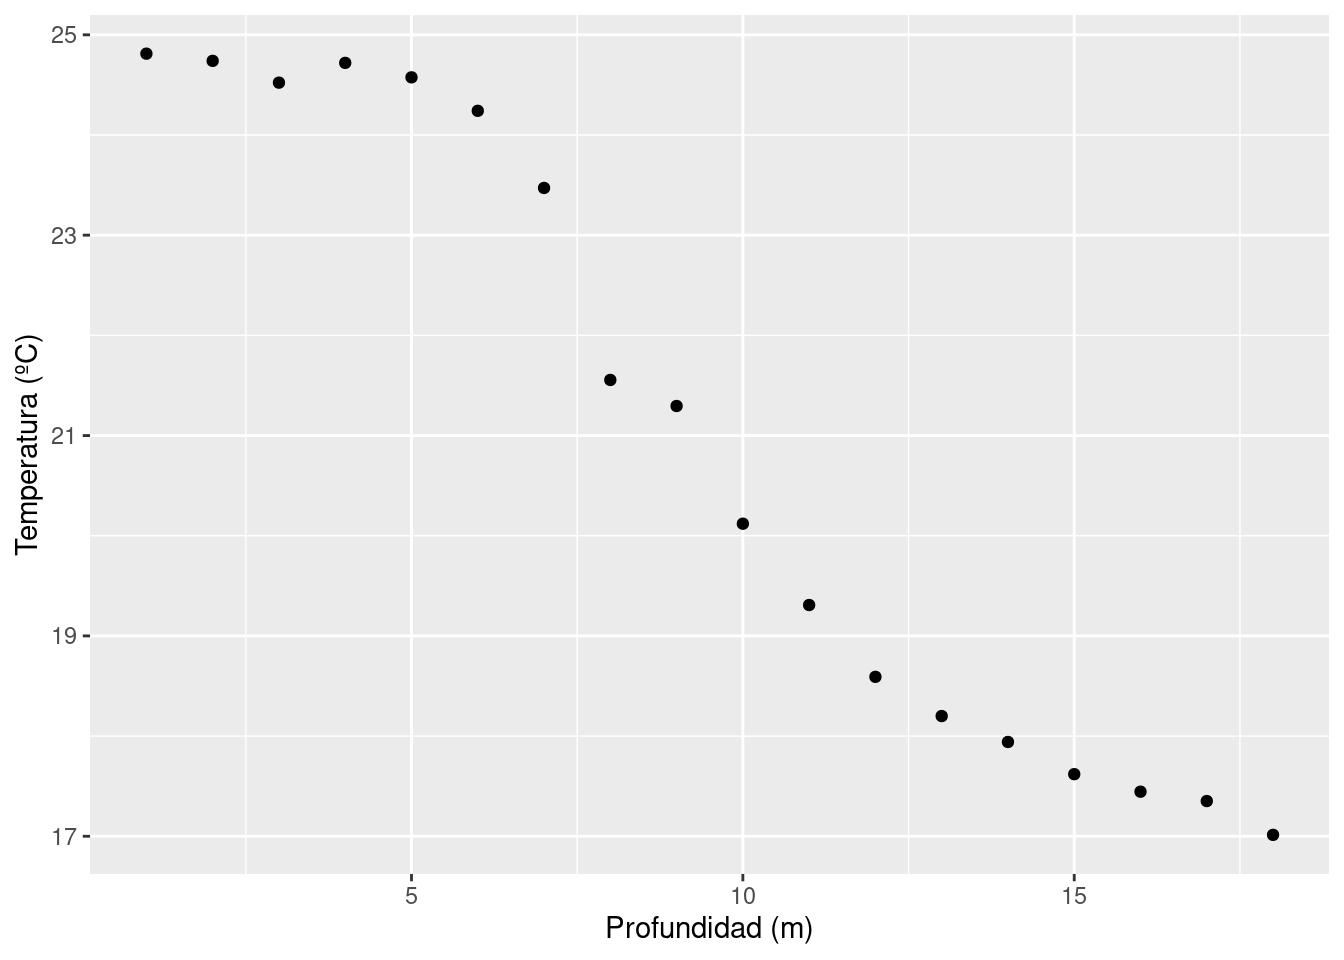
\includegraphics[width=1\linewidth]{Prácticas-Ecología-Sistemas-Acuáticos_files/figure-latex/unnamed-chunk-45-1}

Tiene buena pinta pero es extraño. Nosotr@s estamos acostumbrados a ver los perfiles así:

\begin{figure}

{\centering 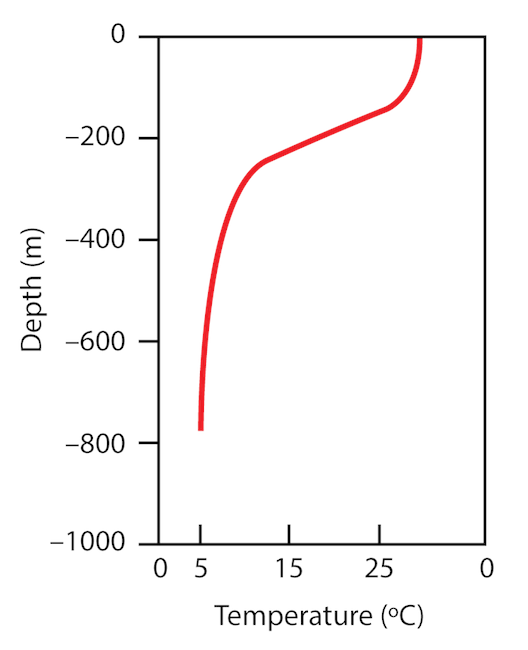
\includegraphics[width=1\linewidth]{Img/Perfil2} 

}

\caption{Representación clásica de un perfil vertical de temperatura.}\label{fig:unnamed-chunk-46}
\end{figure}

Pues vamos a hacer algunos cambios en el código para mejorar esto.

\begin{lstlisting}[language=R]
ggplot(Dia_elegido, aes(y= depth_calculated, x = water_temp))+
  geom_point()+
  scale_y_reverse()+ # Invertimos la profundidad para que la parte superior sea 0 metros.
  scale_x_continuous(position = "top")+ #Colocamos el eje arriba
  labs(x = "Temperatura (ºC)", y = "Profundidad (m)")+
  theme_classic()
\end{lstlisting}

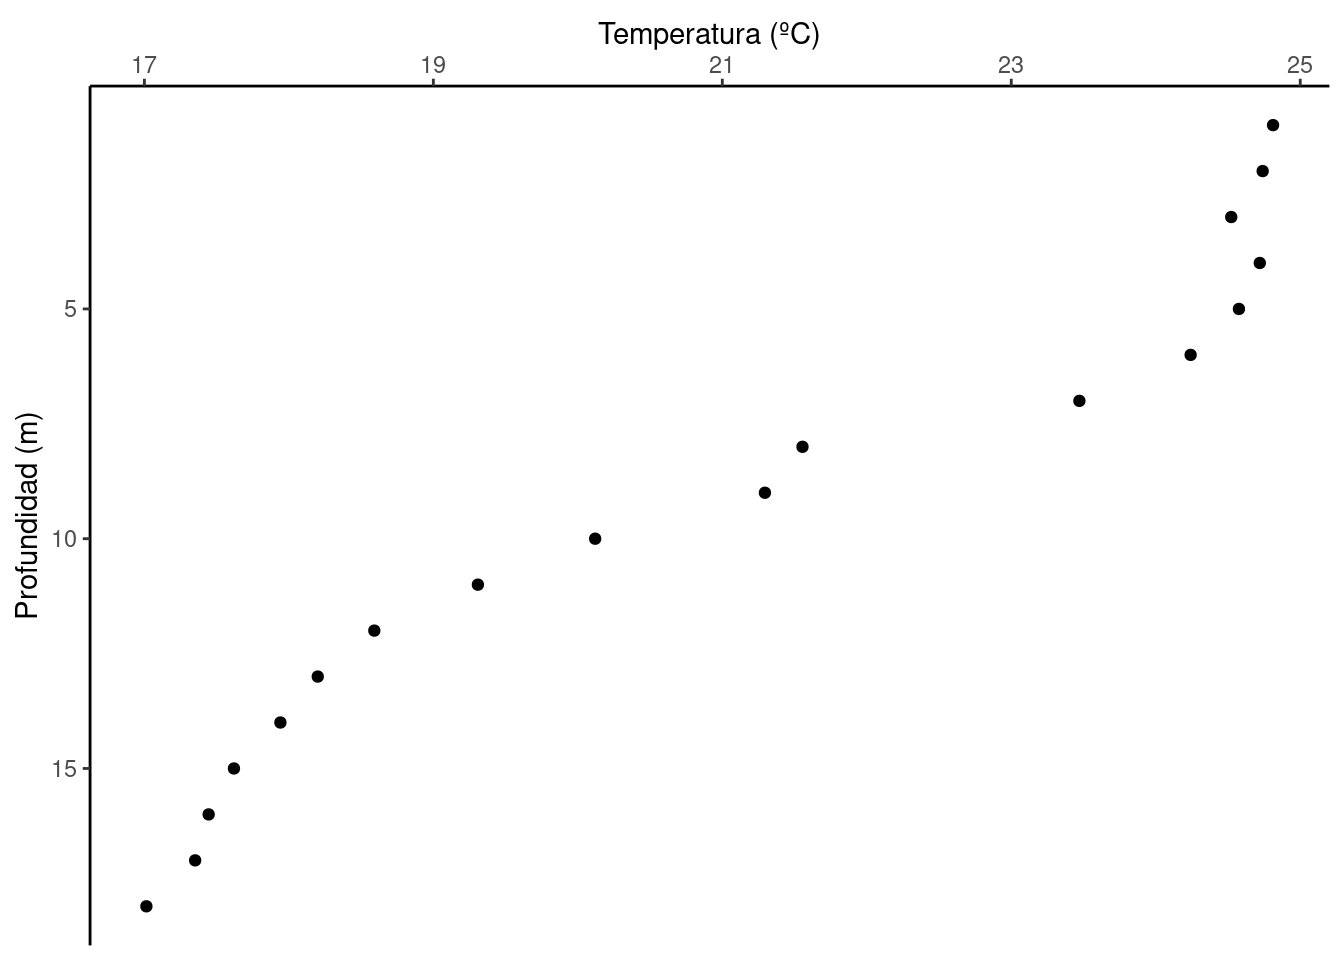
\includegraphics[width=1\linewidth]{Prácticas-Ecología-Sistemas-Acuáticos_files/figure-latex/unnamed-chunk-47-1}

Esto tiene mejor pinta. Prueba a usar \passthrough{\lstinline!geom\_line()!} en lugar de \passthrough{\lstinline!geom\_point()!}. Sucede algo extraño entorno a los 5 metros de profundidad ¿verdad? Esto sucede porque \passthrough{\lstinline!geom\_line()!} une las observaciones ordenadas por la variable \passthrough{\lstinline!x!}. Prueba mejor con \passthrough{\lstinline!geom\_path()!}. Otra opción es asignar la profundidad al eje x y cambiar los ejes (es un poco lioso, os dejo el código por si queréis indagar).

\begin{lstlisting}[language=R]
ggplot(Dia_elegido, aes(x= depth_calculated, y = water_temp))+
  geom_line()+
  coord_flip()+ #Cambia el eje x por el y
  scale_x_reverse()+ # Invertimos la profundidad para que la parte superior sea 0 metros.
  scale_y_continuous(position = "right")+
  labs(x = "Profundidad (m)", y = "Temperatura (ºC)")
\end{lstlisting}

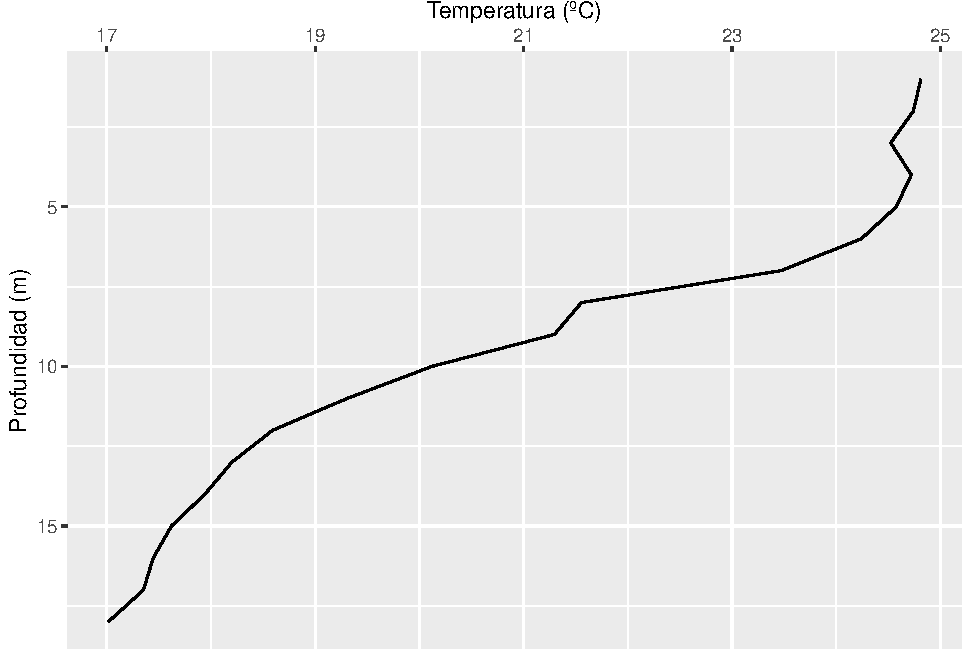
\includegraphics[width=1\linewidth]{Prácticas-Ecología-Sistemas-Acuáticos_files/figure-latex/unnamed-chunk-48-1}

Quitando esta curiosidad con respecto a como se representan las variables, ya tenemos nuestro perfil vertical de temperatura:

\begin{lstlisting}[language=R]
ggplot(Dia_elegido, aes(y= depth_calculated, x = water_temp))+
  geom_path(color = "gray", size = 3)+ #Cambiamos un poco la estética dándole color y grosor a la línea
  scale_y_reverse()+ # Invertimos la profundidad para que la parte superior sea 0 metros.
  scale_x_continuous(position = "top")+ #Colocamos el eje arriba
  labs(x = "Temperatura (ºC)", y = "Profundidad (m)")+
  theme_classic()
\end{lstlisting}

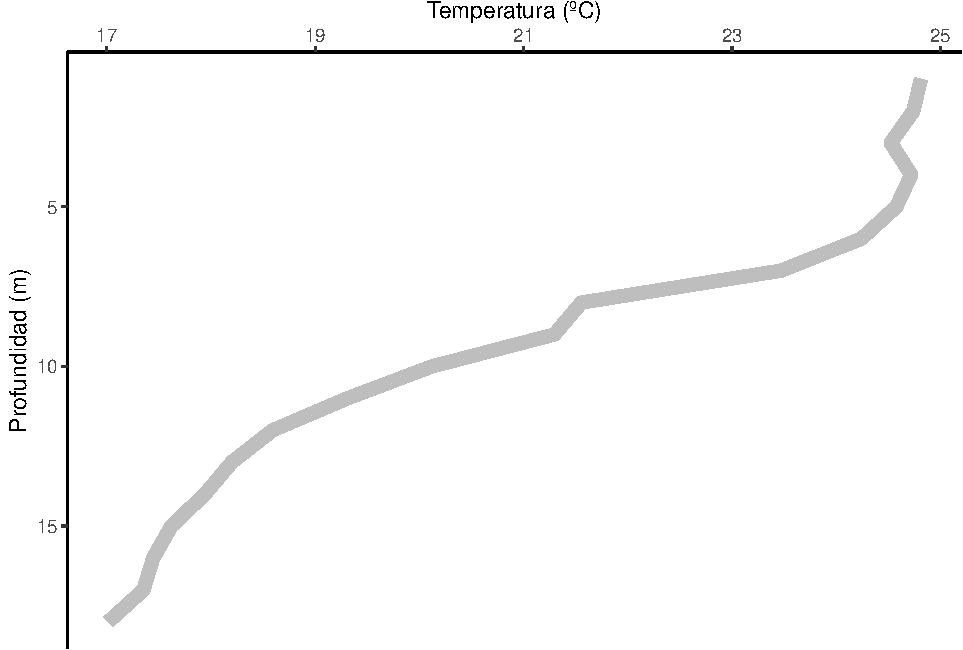
\includegraphics[width=1\linewidth]{Prácticas-Ecología-Sistemas-Acuáticos_files/figure-latex/unnamed-chunk-49-1}

\hypertarget{ejercicio}{%
\subsection{Ejercicio}\label{ejercicio}}

\begin{enumerate}
\def\labelenumi{\arabic{enumi}.}
\tightlist
\item
  \emph{Haz un perfil con la concentración de oxígeno disuelto y otro con el pH.}
\end{enumerate}

\hypertarget{termoclina}{%
\section{Termoclina}\label{termoclina}}

Ahora, en base a el perfil de temperatura que hemos representado, ¿sabrías si este día el lago está estratificado? Si estuviera estratificado, ¿serías capaz de decir a que profundidad se encuentra la termoclina?

A ojo podríamos acercarnos bastante pero imaginad que luego quisiéramos calcularlo para cada día\ldots{} Gracias al altruismo y la ciencia colaborativa tenemos a nuestra disposición un paquete desarrollado especialmente para este tipo de cosas que nos gustan a los limnolog@s. El paquete es \href{https://cran.r-project.org/web/packages/rLakeAnalyzer/rLakeAnalyzer.pdf}{\passthrough{\lstinline!rLakeAnalyzer!}} y contiene métodos estandarizados para calcular propiedades físicas del lago, como la termoclina, la estabilidad de Schmidt, etc. Para instalarlo: \passthrough{\lstinline!install.packages("rLakeAnalyzer")!}. Si echáis un vistazo al paquete veréis un montón de funciones interesantes. Nosotros, ahora mismo, queríamos saber a que profundidad tenemos la termoclina. Para eso, vamos a pedir ayuda para aprender a usar la función \passthrough{\lstinline!?thermo.depth()!}. Aquí podemos ver los argumentos que necesitamos. Por ejemplo, podemos indicarle la densidad mínima para considerar que existe termoclina o la temperatura por debajo de la cual no queremos que calcule termoclina. No vamos a reparar en estos. Sin embargo, el argumento \passthrough{\lstinline!seasonal!} viene por defecto como verdadero, situando la termoclina en el gradiente de densidad más profundo. Nosotros vamos a cambiarlo a \passthrough{\lstinline!FALSE!}. Estos son argumentos opcionales, los indispensables son un vector numérico con la temperatura del agua (\passthrough{\lstinline!wtr!}) y otro vector numérico con la profundidad que corresponde a cada temperatura. Estos los tenemos, así que nos podemos poner manos a la obra:

\begin{lstlisting}[language=R]
#Library
library(rLakeAnalyzer)
#Creamos dos vectors con la información que nos pide
Temp <- Dia_elegido$water_temp
Prof <- Dia_elegido$depth_calculated

#Calculamos la termoclina
thermo.depth(wtr = Temp, depths = Prof, seasonal = FALSE)
\end{lstlisting}

\begin{lstlisting}
## [1] 7.397819
\end{lstlisting}

¡Voilá! Ya tenemos la profundidad a la que está la termoclina. Vamos a representarla:

\begin{lstlisting}[language=R]
#Vamos a guardar la profundidad de la termoclina en un objeto
Termoclina <- thermo.depth(wtr = Temp, depths = Prof, seasonal = FALSE)

ggplot(Dia_elegido, aes(y= depth_calculated, x = water_temp))+
  geom_path(color = "gray", size = 3)+ #Cambiamos un poco la estética dándole color y grosor a la línea
  geom_hline(yintercept = Termoclina)+ #Añadimos la termoclina
  scale_y_reverse()+ # Invertimos la profundidad para que la parte superior sea 0 metros.
  scale_x_continuous(position = "top")+ #Colocamos el eje arriba
  labs(x = "Temperatura (ºC)", y = "Profundidad (m)")+
  theme_classic()
\end{lstlisting}

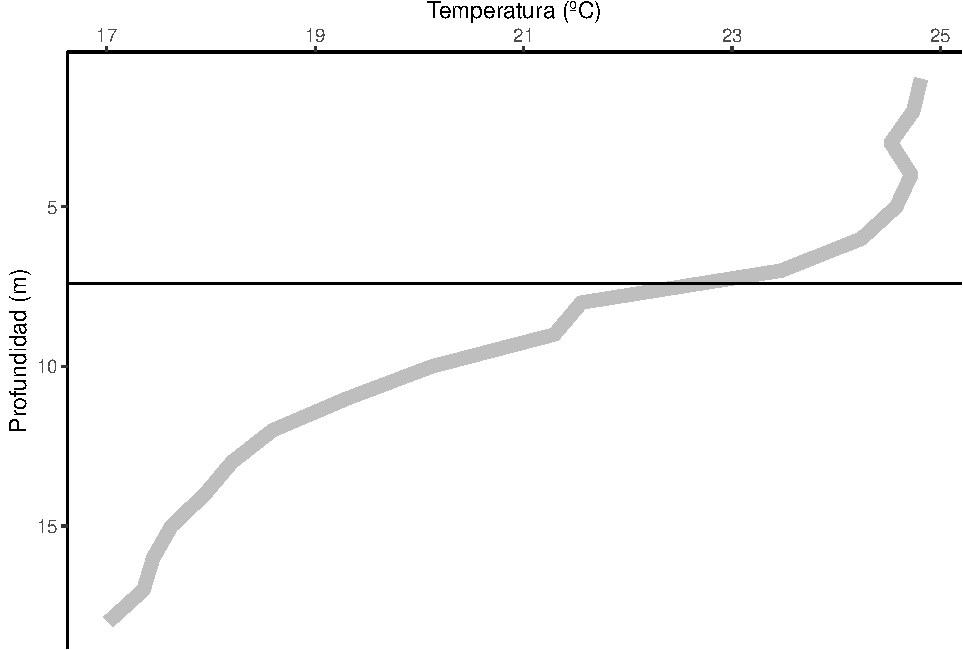
\includegraphics[width=1\linewidth]{Prácticas-Ecología-Sistemas-Acuáticos_files/figure-latex/unnamed-chunk-51-1}

\hypertarget{capas-en-un-lago-estratificado}{%
\section{Capas en un lago estratificado}\label{capas-en-un-lago-estratificado}}

Como sabéis, cuando un lago (o un embalse) se encuentra estratificado se puede diferenciar en distintas capas. Una capa superficial, que está mezclada y en contacto con la atmósfera, el \textbf{epilimnion}, otra capa profunda, aislada de la superior debido al fuerte gradiente de densidad, el \textbf{hipolimnion} y una capa intermedia que hace de interfase entre estas dos capas, el \textbf{metalimnion}. Esto determinan los procesos que tendrán lugar a cada profundidad. La capa superficial al estar en contacto con la atmósfera estará bien oxigenada y dará lugar a que se desarrolle la vida aeróbica sin problemas. La capa profunda, sin embargo, puede acabar volviéndose anóxica y limitando la degradación de la materia orgánica a mecanismos de respiración anaeróbica (desnitrificación, sulfato reducción, etc) y acumulando metales que pueden ser tóxicos y comprometer su uso para abastecimiento humano. Por lo tanto, si estamos estudiando un sistema estratificado es clave reconocer y definir estás capas.

\begin{figure}

{\centering 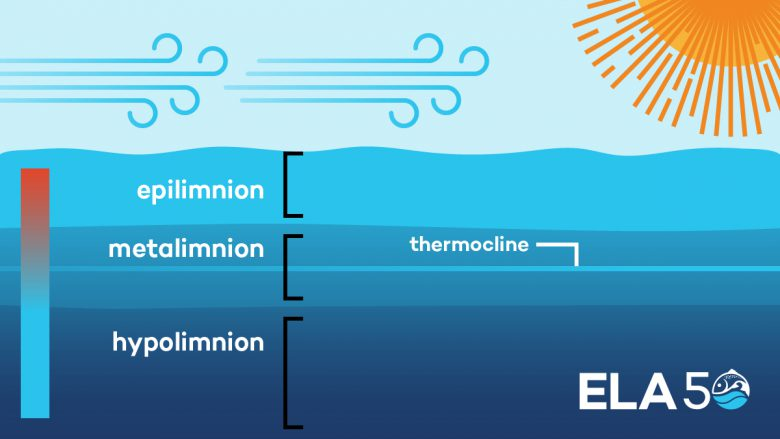
\includegraphics[width=1\linewidth]{Img/Stratified_lake} 

}

\caption{Esquema de un lago estratificado. Fuente: IISD Experimental Lakes Area (IISD-ELA).}\label{fig:unnamed-chunk-52}
\end{figure}

Para determinar donde empiezan y donde acaban estas capas, el paquete \passthrough{\lstinline!rLakeAnalyzer!} dispone de un función, \passthrough{\lstinline!meta.depths()!}. Si leemos la información sobre la función vemos que nos devuelve el límite superior e inferior del metalimnion, que a su vez son el limite inferior del epilimnion y el límite superior del hipolimnion. Además, los argumentos obligatorios son los mismo que usamos con \passthrough{\lstinline!thermo.depth()!}. Así que podemos aplicarla sin problemas.

\begin{lstlisting}[language=R]
meta.depths(wtr = Temp, depths = Prof, seasonal = FALSE)
\end{lstlisting}

\begin{lstlisting}
## [1] 5.654340 8.370172
\end{lstlisting}

¡Perfecto! Vamos a representarlo todo junto.

\begin{lstlisting}[language=R]
#Guardo los límites del metalimnion
metalimnion <- meta.depths(wtr = Temp, depths = Prof, seasonal = FALSE)

ggplot(Dia_elegido, aes(y= depth_calculated, x = water_temp))+
  geom_path(color = "gray", size = 3)+ #Cambiamos un poco la estética dándole color y grosor a la línea
  geom_hline(yintercept = Termoclina)+ #Línea en la termoclina
  geom_hline(yintercept = metalimnion, linetype = 2)+ #Líneas discontinuas defininedo el metalimnion
  scale_y_reverse()+ # Invertimos la profundidad para que la parte superior sea 0 metros.
  scale_x_continuous(position = "top")+ #Colocamos el eje arriba
  labs(x = "Temperatura (ºC)", y = "Profundidad (m)")+
  theme_classic()
\end{lstlisting}

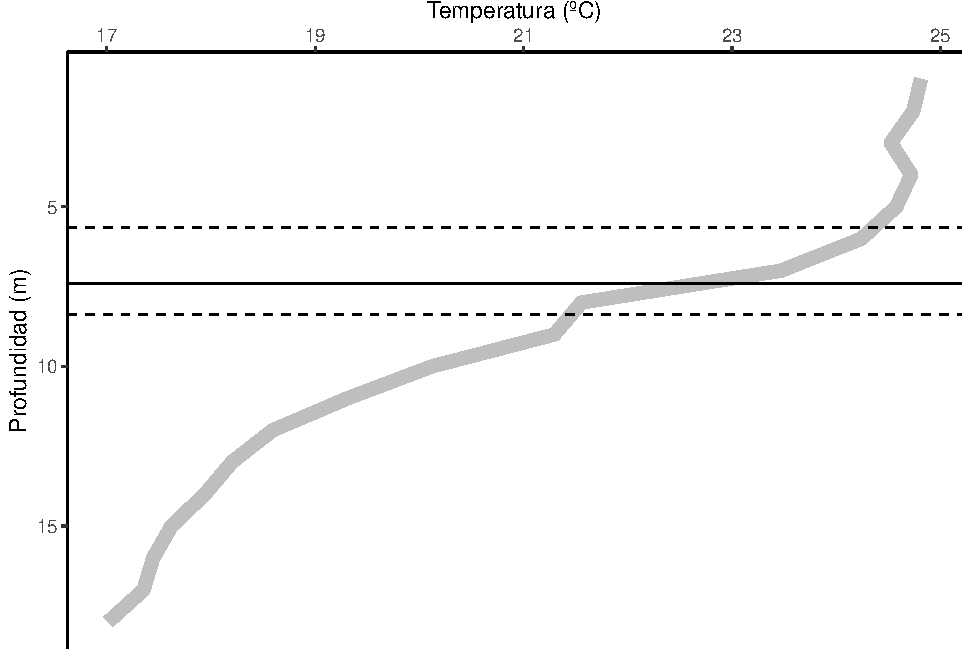
\includegraphics[width=1\linewidth]{Prácticas-Ecología-Sistemas-Acuáticos_files/figure-latex/unnamed-chunk-54-1}

\hypertarget{ejercicios-4}{%
\subsection{Ejercicios}\label{ejercicios-4}}

\begin{enumerate}
\def\labelenumi{\arabic{enumi}.}
\tightlist
\item
  Prueba a cambiar el argumento \passthrough{\lstinline!seasonal!}. ¿Qué sucede?
\item
  ¿Podrías calcular la profundidad de la termoclina para todos los días del año en el lago Crystal?
\end{enumerate}

\hypertarget{estabilidad}{%
\section{Estabilidad}\label{estabilidad}}

La estabilidad de la columna de agua nos va a dar una idea sobre su tendencia a mezclarse o permanecer estratificada. Uno de los índices utilizados para representar la estabilidad de la masa de agua en un lago es el índice de estabilidad de Schmidt. Este indice da un valor sobre la energía que tendríamos que aplicar sobre la superficie para mezclar la columna de agua. Las unidades son, por lo tanto, J/m².

El paquete \passthrough{\lstinline!rLakeAnalyzer!}también nos provee de una función para calcular la estabilidad de Schmidt, \passthrough{\lstinline!schmidt.stability()!}. Echar una ojeada a como se usa.

Si os habéis fijado, en este caso, a parte de la temperatura y la profundidad, necesitamos darle información sobre la batimetría del lago. \passthrough{\lstinline!bthA!} es el área que tiene cada capa a una determinada profundidad \passthrough{\lstinline!bthB!}. Quizás lo veis mejor en la siguiente imagen.

\begin{figure}

{\centering 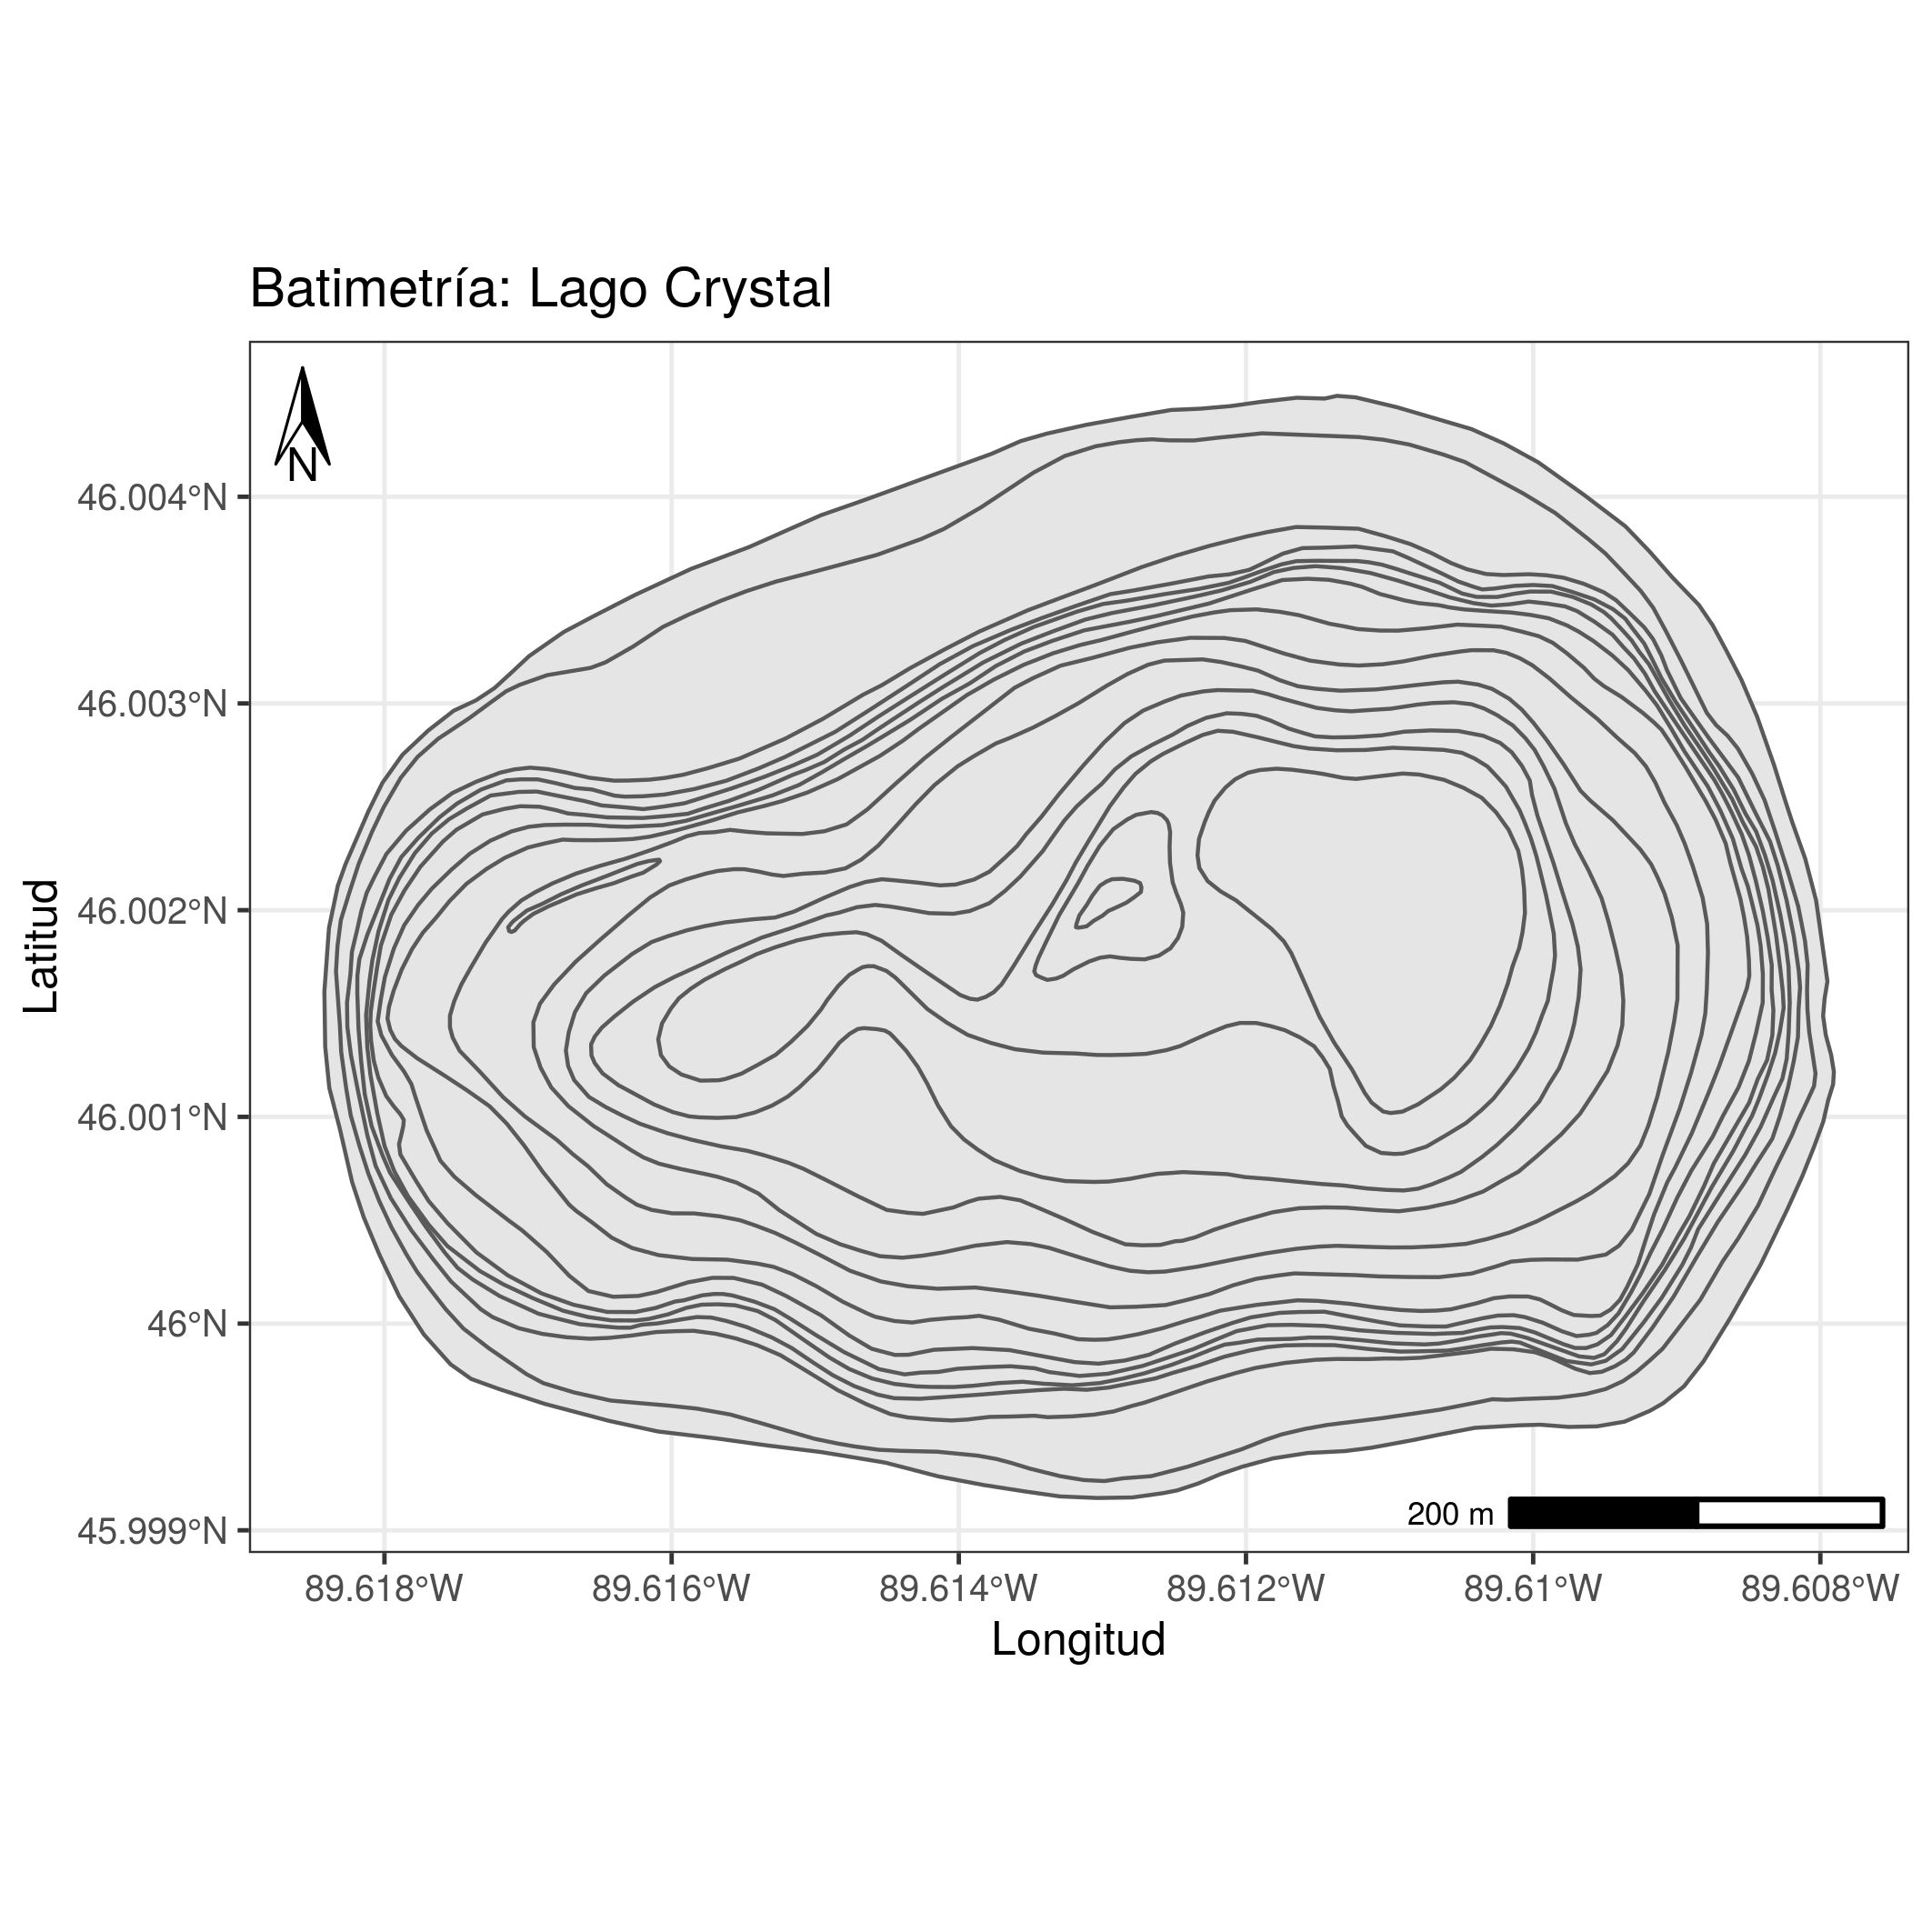
\includegraphics[width=1\linewidth]{Graficas/Lago_crystal_contorno} 

}

\caption{Batimetría del lago Crystal.}\label{fig:unnamed-chunk-56}
\end{figure}

Pues bien, a priori, no disponemos de esta información. Quizás buscando en la base de datos de GLEON podríamos encontrar la batimetría del Lago Crystal. De hecho, está pero en un archivo .shp y deberíamos calcular el área. Todo esto se puede hacer con R (de hecho, la imagen de arriba está hecha con R)pero no vamos a abrir esa puerta ahora, ya tenemos bastante\ldots{}

De nuevo, el paquete \passthrough{\lstinline!rLakeAnalyzer!} nos proporciona la solución a nuestros problemas. Existe una función para estimar la curva área-profundidad (también conocida como curva hipsográfica) para un lago. Sólo tenemos que proporcionarle el área de la superficie del lago, la profundidad máxima y la profundidad media. Toda esta información la tenemos disponible en la página de NTL-LTER (North Temperate Lakes US Long-Term Ecological Research Network). Podéis pinchar \href{https://lter.limnology.wisc.edu/researchsite/crystal-lake}{aquí}. La profundidad máxima es de 20.4 m, la superficie del lago es de 367000 m² y la profundidad media es de 11.4 m. ¡Al lío!

\begin{lstlisting}[language=R]
#Estimamos la batimetría
approx.bathy(Zmax = 20.4, lkeArea = 367000, Zmean = 11.4) 
\end{lstlisting}

\begin{lstlisting}
##    depths   Area.at.z
## 1       0 367000.0000
## 2       1 331901.4802
## 3       2 298566.7051
## 4       3 266995.6747
## 5       4 237188.3891
## 6       5 209144.8481
## 7       6 182865.0519
## 8       7 158349.0004
## 9       8 135596.6936
## 10      9 114608.1315
## 11     10  95383.3141
## 12     11  77922.2414
## 13     12  62224.9135
## 14     13  48291.3303
## 15     14  36121.4917
## 16     15  25715.3979
## 17     16  17073.0488
## 18     17  10194.4444
## 19     18   5079.5848
## 20     19   1728.4698
## 21     20    141.0996
\end{lstlisting}

Ahora ya tenemos toda la información necesaria para calcula la estabilidad de Schmidt.

\begin{lstlisting}[language=R]
#Guardamos la estimación en un objeto
Batimetria <- approx.bathy(Zmax = 20.4, lkeArea = 367000, Zmean = 11.4)

#Calculamos la estabilidad de Schmidt
schmidt.stability(wtr = Temp, depths = Prof, bthA = Batimetria$Area.at.z, bthD =  Batimetria$depths)
\end{lstlisting}

\begin{lstlisting}
##        [,1]
## [1,] 121.69
\end{lstlisting}

La estabilidad de Schmidt para el día 200 es de 121.69 J/m². Este número nos puede decir poco pero\ldots{} ¿y si comparamos distintos días?

\hypertarget{ejercicios-5}{%
\subsection{Ejercicios}\label{ejercicios-5}}

\begin{enumerate}
\def\labelenumi{\arabic{enumi}.}
\tightlist
\item
  \emph{¿Para qué sirve el argumento \passthrough{\lstinline!method!} de la función \passthrough{\lstinline!approx.bathy()!}? ¿Qué efecto tiene?}
\item
  \emph{Vamos a comparar la estabilidad de Schmidt para tres días: el primero que tenemos de 2012, el día 200 y el último que tenemos para 2012.}
\end{enumerate}

\hypertarget{series-temporales}{%
\section{Series temporales}\label{series-temporales}}

Las funciones que hemos visto hasta ahora del paquete \passthrough{\lstinline!rLakeAnalyzer!} las hemos aplicado a perfiles vertical de un día en concreto. En uno de los ejercicios os animé a calcularais la termoclina para cada día del año 2012. Gracias al paquete \passthrough{\lstinline!dplyr!}esta tarea no es realmente complicada. Sin embargo, el paquete \passthrough{\lstinline!rLakeAnalyzer!} posee una versión de cada una de la funciones que hemos visto pero que se puede aplicar a series temporales como la que nosotros tenemos. Echad un vistazo a \passthrough{\lstinline!?ts.thermo.depth!}.
Si os dais cuenta, el único inconveniente en que nos piden una estructura de los datos concreta. Para poder aplicarla tenemos que reorganizar la tabla. La tabla tiene que tener una columna llamada datetime con formato de fecha en lugar de día del año y una columna para cada profundidad.
Lo primero que vamos a hacer es quedarnos solamente con la información del día, de la profundidad y de la temperatura del agua.

\begin{lstlisting}[language=R]
#Seleccionamos las variable que nos interesan
Crystal_temp <- Crystal_dia %>% select(daynum, depth_calculated, water_temp)
\end{lstlisting}

Una vez que hemos seleccionado sólo lo que nos interesa, vamos a convertirlo a forma ancho usando la función \passthrough{\lstinline!spread()!}.

\begin{lstlisting}[language=R]
#Mantenemos la fecha y convertimos la profundidad en variables (columnas) incluyendo el valor de temperatura en cada columna.
Crystal_ts <- Crystal_temp %>% spread(key = depth_calculated, value = water_temp)
\end{lstlisting}

Vamos a convertir el día del año en formato fecha y a cambiarle el nombre a las columnas.

\begin{lstlisting}[language=R]
#Convertimos los días del año en fechas
Crystal_ts <- Crystal_ts %>% mutate_at(vars(daynum), as.Date, origin = "2012-01-01")
#Cambiamos el nombre de la columna "daynum" a "datetime"
Crystal_ts <- Crystal_ts %>% rename(datetime = daynum)
#Añadimos "wtr_" delante del número de cada profundidad
Crystal_ts <- Crystal_ts %>% rename_if(is.numeric, ~paste("wtr_", ., sep = ""))
Crystal_ts
\end{lstlisting}

\begin{lstlisting}
## # A tibble: 189 x 20
##    datetime   wtr_0 wtr_1 wtr_2 wtr_3 wtr_4 wtr_5 wtr_6 wtr_7 wtr_8 wtr_9 wtr_10
##    <date>     <dbl> <dbl> <dbl> <dbl> <dbl> <dbl> <dbl> <dbl> <dbl> <dbl>  <dbl>
##  1 2012-03-23  8.32  6.54  6.41  5.92  5.74  5.66  5.51  5.30  5.14  5.03   4.98
##  2 2012-03-24 NA     7.03  6.79  6.23  5.85  5.79  5.61  5.43  5.29  5.13   5.04
##  3 2012-03-25 NA     7.78  7.12  6.32  6.06  5.90  5.78  5.67  5.42  5.28   5.11
##  4 2012-03-26  8.20  8.11  7.99  7.07  6.04  5.88  5.66  5.60  5.43  5.26   5.06
##  5 2012-03-27 NA     7.18  7.04  7     6.05 NA    NA    NA    NA     5.11   5.13
##  6 2012-03-28 NA     6.50  6.35  6.32  6.30  6.26  6.20  6.16  5.98  5.83   5.46
##  7 2012-03-29 NA     6.36  6.34  6.32  6.31  6.31  6.28  6.12  5.81  5.74   5.69
##  8 2012-03-30  6.02  6.60  6.28  6.25  6.22  6.18  6.16  6.15  6.04  5.98   5.86
##  9 2012-03-31 NA     6.23  6.23  6.21  6.18  6.16  6.15  6.13  6.12  6.12   6.06
## 10 2012-04-01  6.18  6.16  6.10  6.08  6.07  6.06  6.06  6.04  6.04  6.04   6.02
## # ... with 179 more rows, and 8 more variables: wtr_11 <dbl>, wtr_12 <dbl>,
## #   wtr_13 <dbl>, wtr_14 <dbl>, wtr_15 <dbl>, wtr_16 <dbl>, wtr_17 <dbl>,
## #   wtr_18 <dbl>
\end{lstlisting}

Ya tenemos los datos ordenados para aplicar la función \passthrough{\lstinline!ts.thermo.depth()!}. Ahora vamos a intentar calcular la profundidad de la termoclina para cada día.

\begin{lstlisting}[language=R]
termoclina_diaria <- ts.thermo.depth(Crystal_ts)
\end{lstlisting}

Vemos que tenemos muchos días con valor \passthrough{\lstinline!NA!}. Esto se debe a que si la función encuentra un valor de \passthrough{\lstinline!NA!}en el perfil de temperatura devuelve \passthrough{\lstinline!NA!}. Para evitar esto podemos añadir el argumento \passthrough{\lstinline!na.rm = TRUE!}.

\begin{lstlisting}[language=R]
termoclina_diaria <- ts.thermo.depth(Crystal_ts, na.rm = TRUE)
\end{lstlisting}

Ahora vamos a guardar la información en la carpeta \passthrough{\lstinline!Datos!}.

\begin{lstlisting}[language=R]
#Guardamos los perfiles de temperatura de cada día
write_csv(Crystal_ts, "Datos/Crystal_ts.csv")
#Guardamos la profundidad de la termoclina
write_csv(termoclina_diaria, "Datos/Termoclina.csv")
\end{lstlisting}

\hypertarget{ejercicios-6}{%
\subsection{Ejercicios}\label{ejercicios-6}}

\begin{enumerate}
\def\labelenumi{\arabic{enumi}.}
\tightlist
\item
  \emph{Representa la profundidad de la termoclina para cada día.}
\item
  \emph{Calcula la estabilidad de Schmidt para todos los días.}
\item
  \emph{Representa el valor de la estabilidad de Schmidt para cada día.}
\item
  \emph{Calcula los límites del metalimnion para todos los días.}
\end{enumerate}

\hypertarget{Contour}{%
\chapter{Gráficas de contorno}\label{Contour}}

Por último y aprovechando que tenemos información diaria de la temperatura del lago a distintas profundidades, quizás, sería interesante realizar una gráfica de contorno del periodo estudiado. Estas gráficas son muy visuales y ayudan a entender mejor el comportamiento del lago. Las vemos a menudo en los artículos.

\begin{figure}

{\centering 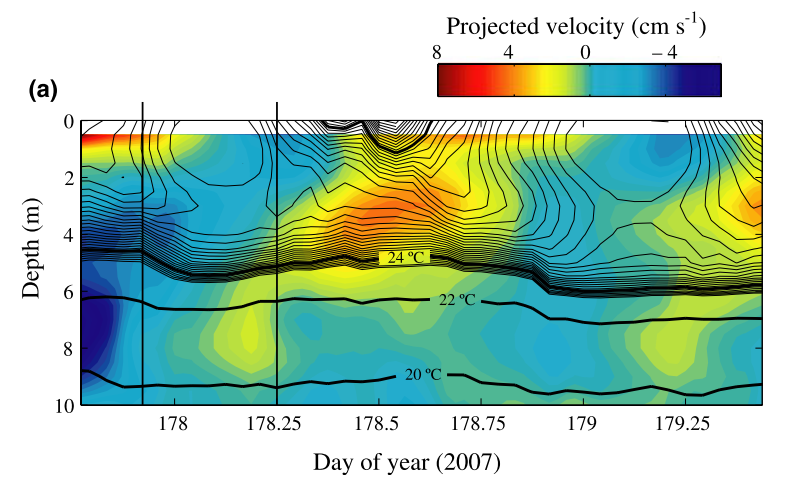
\includegraphics[width=1\linewidth]{Img/Imagen_ContourPlot} 

}

\caption{Imagen ejemplo de gráfica de contorno extraída de @Vidal2010.}\label{fig:unnamed-chunk-66}
\end{figure}

Existen distintos programas que permiten hacer estas gráficas como son Surfer, SigmaPlot o OceanDataView, con el inconveniente que la mayoría de ellos son privativos y de pago (OceanDataView se salva!). Además, ya estamos metidos en harina y, como hemos dicho anteriormente, R nos permite trabajar desde los datos crudos hasta la generación de gráficas e informes (estos documentos están hechos directamente desde R).

Vamos a partir de la tabla de datos en formato ``ancho'' que creamos para calcular la profundidad de la termoclina \passthrough{\lstinline!Crystal\_ts!}.

\begin{lstlisting}[language=R]
#Cargamos tidyverse si cerramos la sesión anterior
library(tidyverse)
#Importamos los datos de temperatura
Crystal_ts <- read_csv("Datos/Crystal_ts.csv")
\end{lstlisting}

\begin{lstlisting}
## 
## -- Column specification --------------------------------------------------------
## cols(
##   .default = col_double(),
##   datetime = col_date(format = "")
## )
## i Use `spec()` for the full column specifications.
\end{lstlisting}

Cuando transformamos el objeto a formato ``ancho'' homogeneizamos las profundidades a las que tenemos datos de temperatura. Es decir, tenemos el mismo número de medidas y a las mismas profundidades para cada momento. Sin embargo, como los datos no estaban completos se han introducidos NAs en aquellas profundidades donde no teníamos información. Por ejemplo, en el perfil del 2012-03-27, tenemos datos de temperatura a 4 y a 9 metros pero no para las profundidades entre 5-8 m. Para solucionar esto, podemos interpolar los datos. Para ello, vamos a usar un nuevo paquete, \href{https://cran.r-project.org/web/packages/zoo/zoo.pdf}{\passthrough{\lstinline!zoo!}}.

\begin{lstlisting}[language=R]
#Cargamos el paquete. Tiene que estar previamente instalado
library(zoo)
\end{lstlisting}

\begin{lstlisting}
## 
## Attaching package: 'zoo'
\end{lstlisting}

\begin{lstlisting}
## The following objects are masked from 'package:base':
## 
##     as.Date, as.Date.numeric
\end{lstlisting}

\begin{lstlisting}[language=R]
#Interpolamos y extrapolamos (rule = 2) la temperatura para las profundidades que nos faltan.
  Crystal_ts[,-1] <- na.approx(Crystal_ts[,-1],rule = 2)
\end{lstlisting}

Ahora podemos devolver los datos a su formato largo.

\begin{lstlisting}[language=R]
#Cargamos el paquete tidyverse
  library(tidyverse)
#Devolvemos la tabla al formato "largo"
  Temp_largo <- gather(Crystal_ts, key = "depth", value = "wtemp", -datetime)
#Le quitamos "wtr_" a la variable profundidad para que se quede sólo los números.
  Temp_largo <- Temp_largo %>% mutate(depth = parse_number(depth))
\end{lstlisting}

E intentamos representar.

\begin{lstlisting}[language=R]
ggplot(Temp_largo, aes(x = datetime, y = depth, color = wtemp))+
  geom_point()
\end{lstlisting}

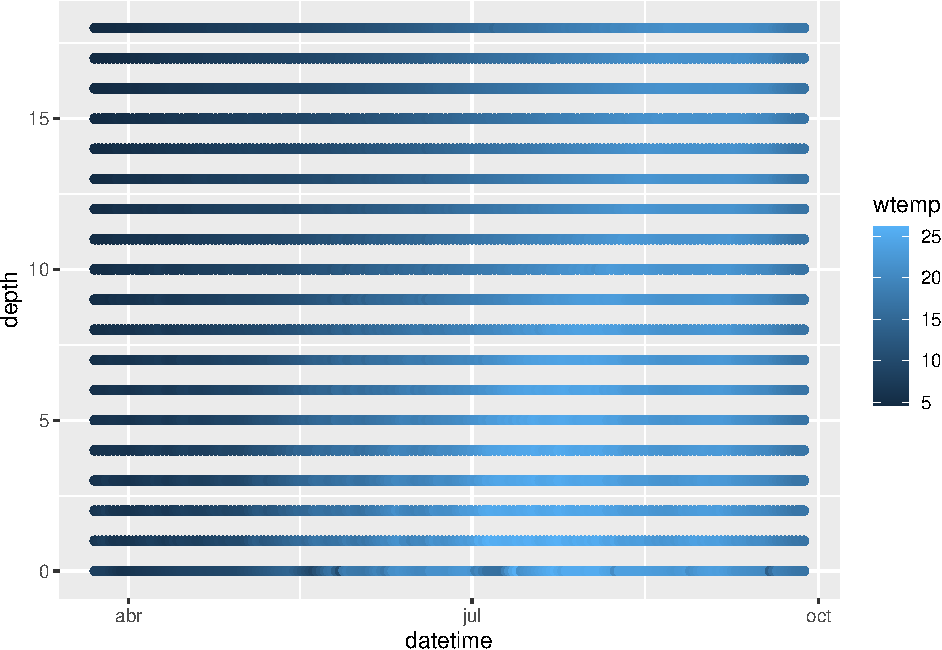
\includegraphics[width=1\linewidth]{Prácticas-Ecología-Sistemas-Acuáticos_files/figure-latex/unnamed-chunk-71-1}

Parece que estamos bastante cerca, sin embargo, hay muchos huecos en blanco. Para solucionar esto vamos a crear una matriz y a usar una interpolación espacial multinivel b-spline para completar la información que nos falta. Para esto, usamos el paquete \href{https://cran.r-project.org/web/packages/MBA/MBA.pdf}{MBA}.

\begin{lstlisting}[language=R]
#Cargamos lubridate, aunque viene con tidyverse hay que "llamarlo" a parte.
  library(lubridate)
#Primero tenemos que convertir las fechas en un vector numérico
  Temp_largo$datetime <- decimal_date(Temp_largo$datetime)
#Cargamos el paquete MBA, hay que instalarlo previamente.
  library(MBA)
# Aquí creamos una matriz con mayor resolución usando una interpolación espacial multinivel b-spline
Temp_mba <- mba.surf(Temp_largo, no.X = 500, no.Y = 500, extend = T)
#Aquí están las fecha con la nueva resolución (en este caso es mayor de la que teniamos, 500 "perfiles", frente a los 189 que teníamos)
head(Temp_mba$xyz.est$x)
\end{lstlisting}

\begin{lstlisting}
## [1] 2012.224 2012.225 2012.226 2012.227 2012.228 2012.229
\end{lstlisting}

\begin{lstlisting}[language=R]
#Aquí tenemos las nuevas profundidades, 500 profundidades en lugar de las 19 que teniamos antes
head(Temp_mba$xyz.est$y)
\end{lstlisting}

\begin{lstlisting}
## [1] 0.00000000 0.03607214 0.07214429 0.10821643 0.14428858 0.18036072
\end{lstlisting}

\begin{lstlisting}[language=R]
#Estos son los datos de temperatura
head(Temp_mba$xyz.est$z)[1:10]
\end{lstlisting}

\begin{lstlisting}
##  [1] 8.336292 8.334450 8.329062 8.320237 8.308084 8.290180 8.312388 8.310018
##  [9] 8.303618 8.293271
\end{lstlisting}

\begin{lstlisting}[language=R]
#Los juntamos todos
Temp_prof <- as.data.frame(Temp_mba$xyz.est$z)
colnames(Temp_prof) <-  Temp_mba$xyz.est$y
Temp_prof <- bind_cols(date = Temp_mba$xyz.est$x, Temp_prof)
#Y los volvemos al formato largo.
Temp_mba <- gather(Temp_prof, key = "depth", value = 'temp', -date) %>%  mutate(temp = round(temp, 3))

#Ponemos la profundidad en numérico, se nos había quedado como carácter
Temp_mba <- Temp_mba %>% mutate(depth = as.numeric(depth))

#Esta es la pinta de los datos:
head(Temp_mba)
\end{lstlisting}

\begin{lstlisting}
##       date depth  temp
## 1 2012.224     0 8.336
## 2 2012.225     0 8.334
## 3 2012.226     0 8.329
## 4 2012.227     0 8.320
## 5 2012.228     0 8.308
## 6 2012.229     0 8.290
\end{lstlisting}

Ahora representamos de nuevo.

\begin{lstlisting}[language=R]
ggplot(Temp_mba, aes(x = date, y = depth, color = temp))+
  geom_point()
\end{lstlisting}

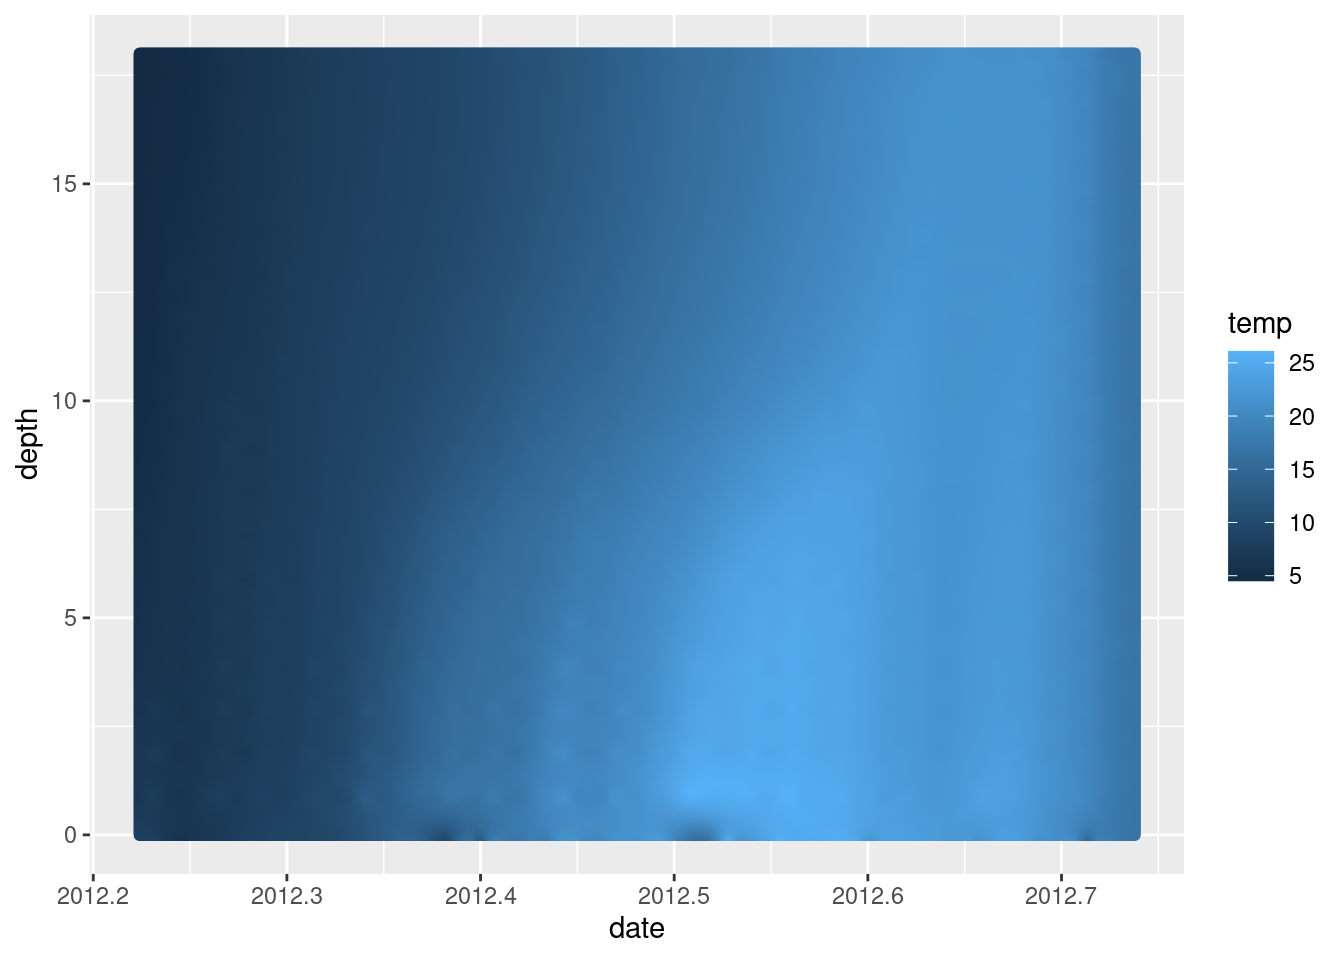
\includegraphics[width=1\linewidth]{Prácticas-Ecología-Sistemas-Acuáticos_files/figure-latex/unnamed-chunk-73-1}

¡Mucho mejor! Vamos a cambiar algunos aspectos estéticos para que quede más resultona.

\begin{lstlisting}[language=R]
#Vamos a devolverle el formato de fecha
Temp_mba$date <- date_decimal(Temp_mba$date)
#Cargamos un paquete para usar una paleta de color má común
library(colorRamps)
Grafica_temp <- ggplot(data = Temp_mba, aes(x = date, y = depth)) +
  geom_tile(aes(fill = temp)) + #Usamos esta capa que viene mejor para este tipo de gráficos pero podíamos haber usado geom_point
  scale_y_reverse()+
  scale_fill_gradientn(colours = matlab.like2(10)) +
  geom_contour(aes(z = temp), binwidth = 1, colour = "black", alpha = 0.2) +
  labs(y = "Profundidad (m)", x = NULL, fill = "temp. (°C)") +
  coord_cartesian(expand = 0)
Grafica_temp
\end{lstlisting}

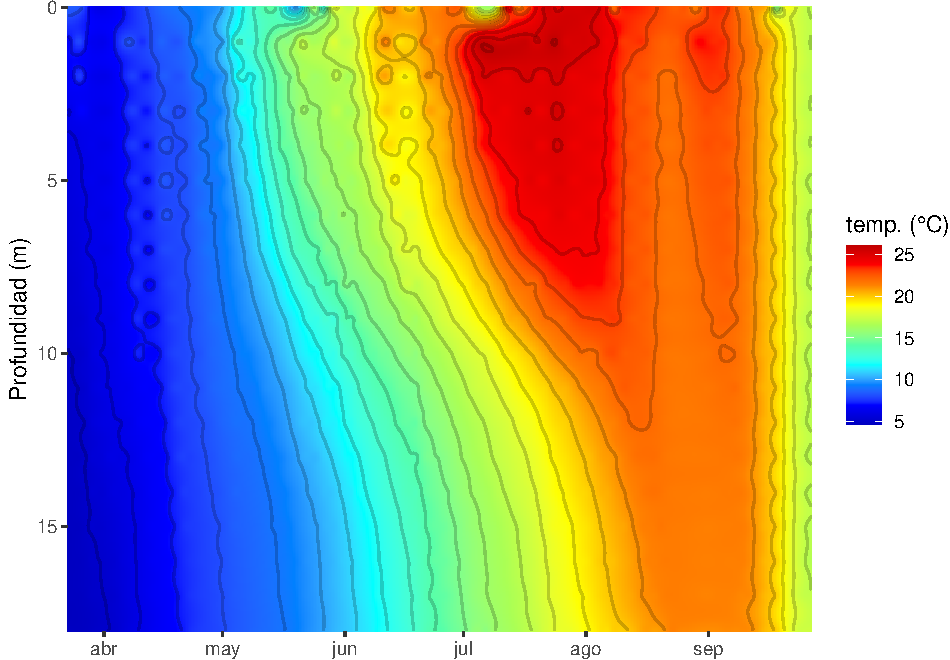
\includegraphics[width=1\linewidth]{Prácticas-Ecología-Sistemas-Acuáticos_files/figure-latex/unnamed-chunk-74-1}

Hemos cambiado el formato de la fecha, hemos invertido el eje profundidad para que se más intuitivo, hemos cambiado las etiquetas, el color y añadido unas lineas de contorno.

Vamos a probar a añadirle la profundidad de la capa de mezcla.

\begin{lstlisting}[language=R]
Termoclina <- read_csv("Datos/Termoclina.csv")
\end{lstlisting}

\begin{lstlisting}
## 
## -- Column specification --------------------------------------------------------
## cols(
##   datetime = col_date(format = ""),
##   thermo.depth = col_double()
## )
\end{lstlisting}

\begin{lstlisting}[language=R]
  Grafica_temp_zmix <- Grafica_temp + geom_line(data = Termoclina, aes(x=datetime, y = thermo.depth, color = "Termoclina"), size = 0.2)+
  scale_color_manual(values = "black") + labs(color = NULL)
  
  Grafica_temp_zmix
\end{lstlisting}

\begin{lstlisting}
## Error: Invalid input: time_trans works with objects of class POSIXct only
\end{lstlisting}


\includegraphics[width=1\linewidth]{Prácticas-Ecología-Sistemas-Acuáticos_files/figure-latex/unnamed-chunk-75-1}

¡Vaya! Tenemos un error. Esto saca de quicio pero os iréis acostumbrando, poco a poco empezaréis a comprender que quiere decir el mensaje de error y buscar en qué os habéis equivocado. En este caso, el error nos dice que al transforma un objeto de tiempo no ha podido porque trabaja con objetos de clase POSIXct. Si os fijáis en el data.frame que usamos para hacer la gráfica de contorno (\passthrough{\lstinline!Temp\_mba!}) la fecha está en formato \passthrough{\lstinline!POSIXct!} y en el data.frame de \passthrough{\lstinline!Termoclina!} está en formato \passthrough{\lstinline!Date!}. Sólo tenemos que cambiar el formato de este último y estará solucionado.

\begin{lstlisting}[language=R]
Termoclina <- Termoclina %>% mutate(datetime = as.POSIXct(datetime))

Grafica_temp_zmix <- Grafica_temp + geom_line(data = Termoclina, aes(x=datetime, y = thermo.depth, color = "Termoclina"), size = 0.2)+
  scale_color_manual(values = "black") + labs(color = NULL)
  
  Grafica_temp_zmix
\end{lstlisting}

\begin{lstlisting}
## Warning: Removed 9 row(s) containing missing values (geom_path).
\end{lstlisting}

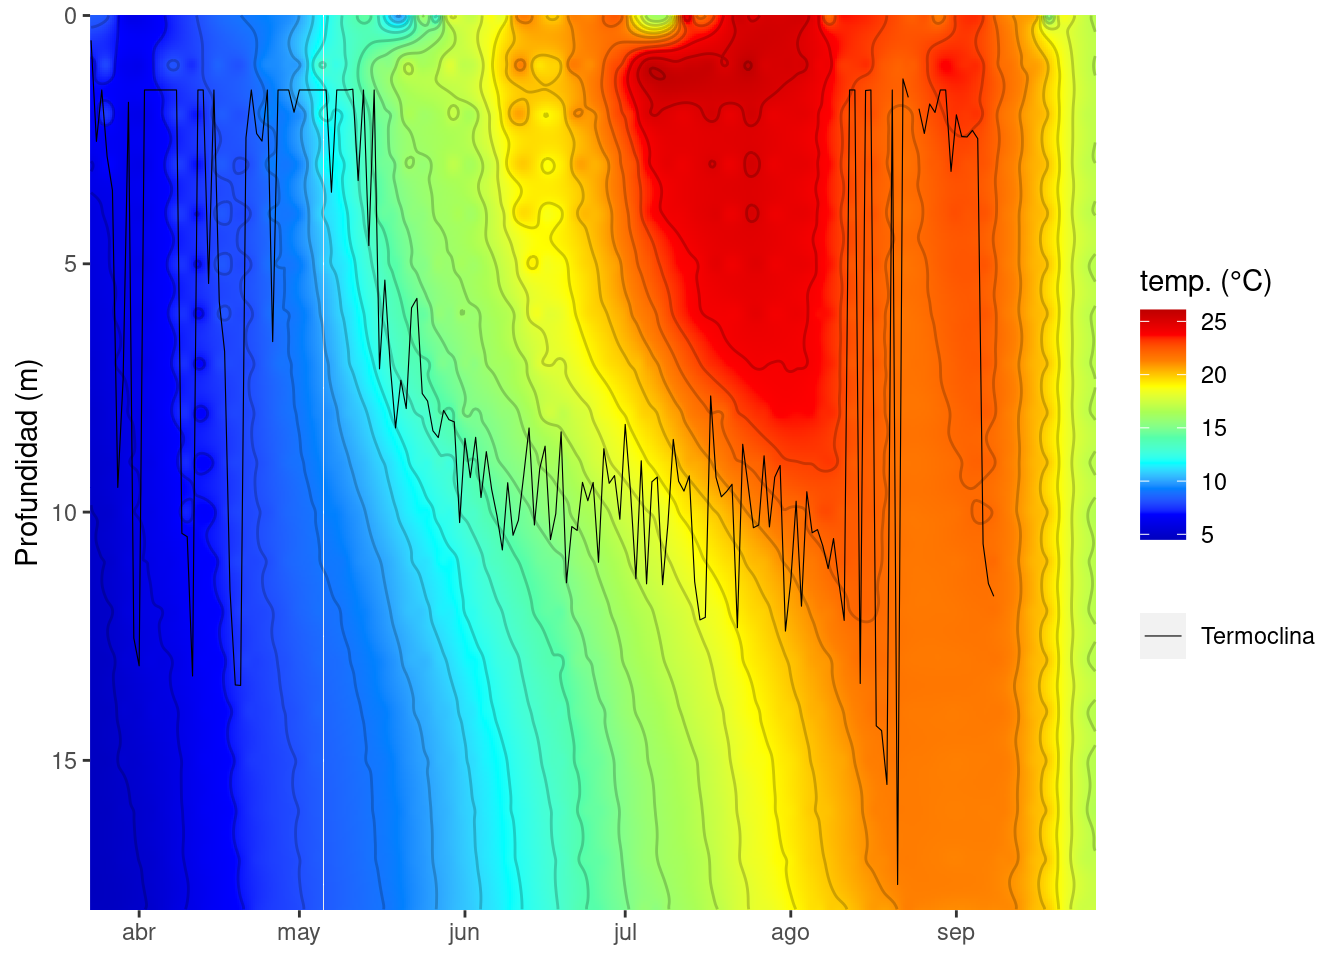
\includegraphics[width=1\linewidth]{Prácticas-Ecología-Sistemas-Acuáticos_files/figure-latex/unnamed-chunk-76-1}

Como vemos hay cierta oscilación en la termoclina y sobretodo en los momentos en lo que la estratificación está comenzando o se está rompiendo. A rasgos generales podemos decir que la estratificación comienza a finales de mayo y se prolonga hasta mediados de agosto. A mediados de agosto vemos que se rompe la estratificación y vuelve a estratificarse suavemente pero a mediados de septiembre el lago está totalmente mezclado con las isotermas totalmente verticales. Si queremos, para visualizar la termoclina podemos usar un suavizado:

\begin{lstlisting}[language=R]
Grafica_temp_zmix <- Grafica_temp + geom_smooth(data = Termoclina, aes(x=datetime, y = thermo.depth, color = "Termoclina"), size = 0.2, na.rm = TRUE, se = FALSE)+
  scale_color_manual(values = "black") + labs(color = NULL)
  
  Grafica_temp_zmix
\end{lstlisting}

\begin{lstlisting}
## `geom_smooth()` using method = 'loess' and formula 'y ~ x'
\end{lstlisting}

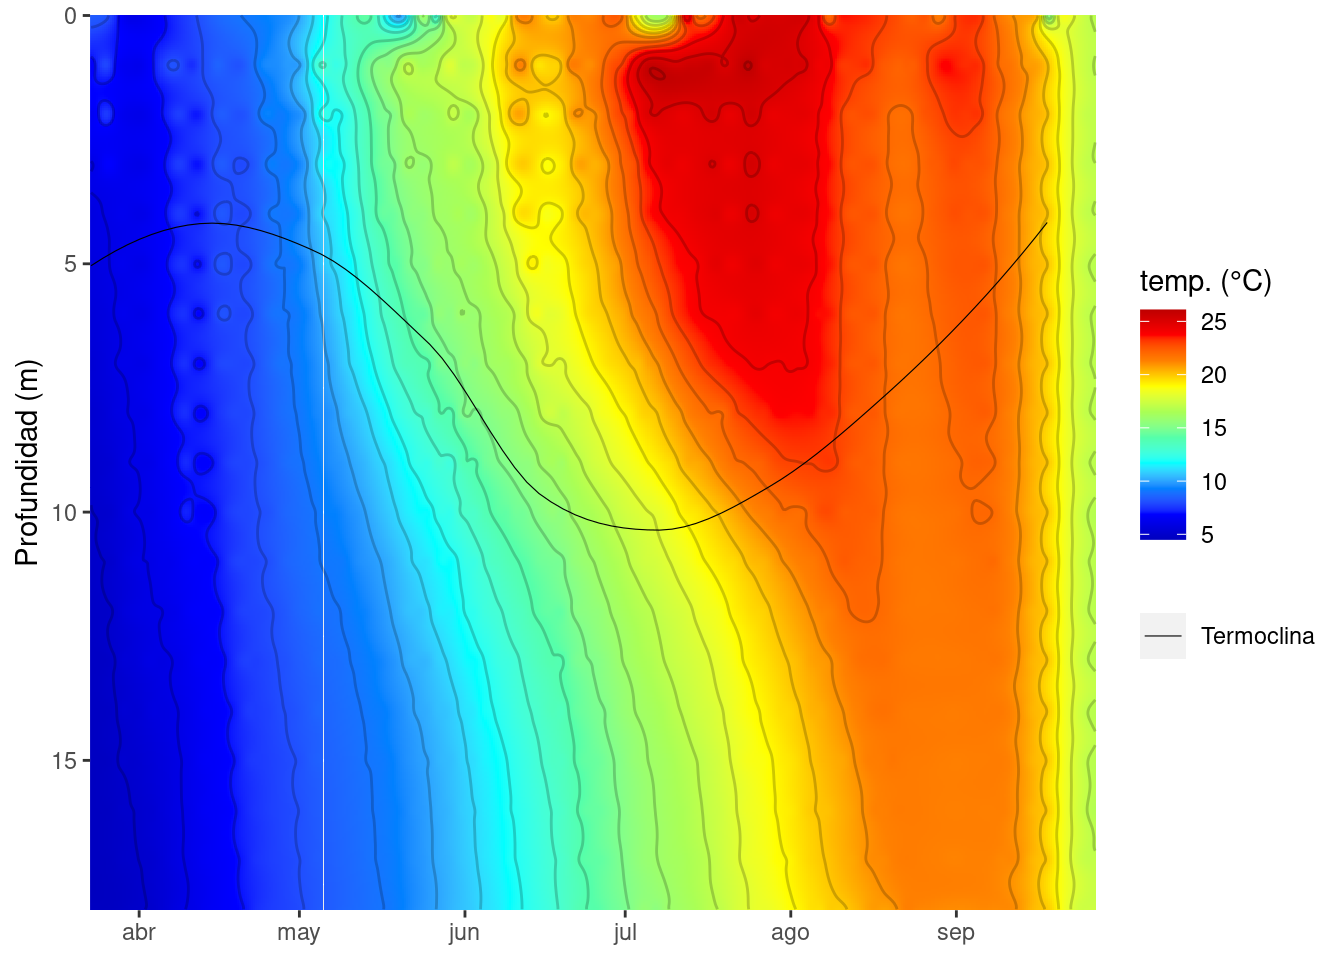
\includegraphics[width=1\linewidth]{Prácticas-Ecología-Sistemas-Acuáticos_files/figure-latex/unnamed-chunk-77-1}

Y ya la tenemos lista para exportar. Podéis guardarla en el formato que más os guste (.jpeg, .pdf, .bmp, \ldots) simplemente cambiando el nombre con el que lo guardáis o indicándolo con el argumento \passthrough{\lstinline!device!}. Además también podéis fijar el ancho y el largo, así como otras opciones que podéis ver en \passthrough{\lstinline!?ggsave()!}.

\begin{lstlisting}[language=R]
ggsave("./Graficas/Grafica_temp.png", Grafica_temp_zmix, width = 20, height = 10, units = "cm")
\end{lstlisting}

\hypertarget{ejercicios-7}{%
\subsection{Ejercicios}\label{ejercicios-7}}

\begin{enumerate}
\def\labelenumi{\arabic{enumi}.}
\tightlist
\item
  \emph{Añade el límite superior e inferior del metalimnion a la gráfica \passthrough{\lstinline!Gráfica\_temp!}.}
\item
  \emph{Haz una gráfica de contorno para el oxígeno disuelto.}
\end{enumerate}

\backmatter

  \bibliography{Mi\_Bibliografia.bib}

\end{document}
